\documentclass[beamer, xcolor={table,usenames,dvipsnames}]{beamer}
%\usepackage{mathpazo}
\usepackage[T1]{fontenc}
\usepackage[utf8]{inputenc}
\usepackage[ngerman]{babel}
\usepackage[babel,german=quotes]{csquotes}
\usepackage{lmodern} % for removing warning about font shape

%\usetheme{Madrid}
\usetheme{Frankfurt}
%\usetheme{Singapore}
\usecolortheme{crane}

\setbeamertemplate{footline}[frame number] % für Foliennummerierung
\beamertemplatenavigationsymbolsempty % Navigationsleiste 

\AtBeginSection{\frame{\sectionpage}}
\newtranslation[to=ngerman]{Section}{Abschnitt}
\newtranslation[to=ngerman]{Subsection}{Beispielmodell}

\usepackage{etoolbox}
\makeatletter
\patchcmd{\slideentry}{\ifnum#2>0}{\ifnum2>0}{}{\@error{unable to patch}}% replace the subsection number test with a test that always returns true
\makeatother

%\setbeameroption{show notes}

\usepackage{amsmath}
\usepackage{calc}

\usepackage{graphicx} %Zum Einbinden von Grafikdateien
\usepackage[font={footnotesize, sf}]{caption}
\usepackage{subfig}
\graphicspath{{./Abbildungen/}}

\usepackage{booktabs} %Für schönere Tabellen
\usepackage{xspace}

\usepackage{tikz} %Für Skizzen

\usepackage[bibstyle=authortitle, citestyle=authortitle, isbn=false, doi=false,
dashed=false]{biblatex}
\addbibresource{Masterarbeit.bib}
\renewbibmacro*{cite:title}{%
  \printtext[bibhyperref]{%
    \printfield[citetitle]{labeltitle}%
    \setunit{\addcomma\space}%
    \printdate}}

%\usepackage{vmargin} %Fürs Seitenlayout
%\setmarginsrb{2.5cm}{1.5cm}{2cm}{1.5cm}{0mm}{0.5cm}{0mm}{1cm}

%%% Häkchen und Kreuzchen %%%
\usepackage{pifont}% http://ctan.org/pkg/pifont
\newcommand{\cmark}{\ding{51}}%
\newcommand{\xmark}{\ding{55}}%

\usepackage{todonotes}

%%% Eigene Befehle %%%
\newcommand{\was}[1]{\small\textit{#1}}
\newcommand{\noteS}[1]{\todo[color=green!40]{\textbf{Sascha: }#1}}
\newcommand{\noteJ}[1]{\todo[color=blue!40]{\textbf{János: }#1}}
\newcommand{\textfrac}[2]{\hspace{2pt} \frac{\text{#1}}{\text{#2}}}
\newcommand{\eqnref}[1]{\overset{(\ref{#1})}{=}} % Gleichheitszeichen mit Referenz auf die verwendete Gleichung
\newcommand{\defeq}{\vcentcolon=} %Definitions-Gleichheitszeichen
\newcommand{\eqdef}{=\vcentcolon}
\newcommand{\pfrac}[2]{\frac{\partial #1}{\partial #2}}
\newcommand{\markera}[1]{\textcolor{NavyBlue}{#1}} % Farbiger Text 1
\newcommand{\markerb}[1]{\textcolor{Orange}{#1}} % Farbiger Text 2

% Formeln:
\newcommand{\MIPS}[1][]{
  \ifthenelse {\equal {#1} {}}
  {\text{MIPS}} % if argument is blank
  {\text{MIPS}({#1})} % if an optional argument is given
}
\renewcommand{\P}[1]{P_\text{#1}}
\newcommand{\I}[1]{I_\text{#1}}
\newcommand{\itext}[1]{i_\text{#1}}
\newcommand{\T}[1]{T_\text{#1}}
\newcommand{\n}[1]{n_\text{#1}}
\newcommand{\N}[1]{N_\text{#1}}
\renewcommand{\t}[1]{t_\text{#1}}



\title{Ökologische Nachhaltigkeit durch \\ \enquote{Nutzen statt Besitzen}?}
\subtitle{{\small Entwicklung eines Modells zur Ableitung von Kriterien für die Senkung des Umweltverbrauchs durch gemeinschaftliche Produktnutzung}}
\author{Alexander Müller, János Sebestyén}
\date{Universität Osnabrück, 14.07.2015}

\begin{document}

\frame[plain]{\titlepage}


\begin{frame}[plain]
    \begin{center}
        \makebox[\textwidth]{
        \includegraphics<1>[width=\paperwidth]{Luhrmannhof.jpg}
        \includegraphics<2>[width=\paperwidth]{Luhrmannhof50.pdf}
        \includegraphics<3>[width=\paperwidth]{Luhrmannhof50x2.pdf}
        \includegraphics<4>[width=\paperwidth]{Luhrmannhof10x5.pdf}}
    \end{center}
\end{frame}
\frame<beamer>{\tableofcontents}
\section{Einleitung}

\subsection{Thema}
	\begin{frame}{Thema}
        \begin{itemize}
            \item Gemeinschaftliche Nutzung von Produkten \\ Waschsalon,
                Car-Sharing, Werkzeugverleih,\dots
            \item Ökologische Auswirkungen solcher Nutzungsformen im Vergleich
                zur individuellen Nutzung
        \end{itemize}
        	\begin{center}
        		\small
        		\begin{tabular}{p{5cm}p{5cm}}
        			\multicolumn{2}{l}{\textbf{Umwelteffekte durch die
        					Nutzung}}  \\[5pt]
        			\textbf{positiv} & \textbf{negativ} \\
        			\midrule
        			Nutzungsintensivierung  &  Zusätzliche Transporte
        			\\[3pt]
        			Erhöhung der Produktauslastung  & Erhöhung der Produktauslastung \\[3pt]
        			Wartung / Reparaturen &  Wartung / Reparaturen \\[3pt]
        			\bottomrule
        		\end{tabular}
        		\vspace{3pt}

        		Für vollständige Übersicht siehe \cite{scholl_marketing_2009}.
        \end{center}
	\end{frame}



    \subsection{Fragestellung}
	\begin{frame}{Fragestellung}
      \begin{block}{}
	        	\begin{itemize}
	        		\item[] Unter welchen Umständen kann der \textit{Umweltverbrauch} eines Produktes durch gemeinschaftliche Nutzung gegenüber der individuellen Nutzung gesenkt werden?
	        		% \item Was sind die Mechanismen, die den Umweltverbrauch bei gemeinschaftlicher Nutzung bestimmen und wie wirken diese? 
	        		% \item Welche Eigenschaften des Produkts und der Nutzungsform beeinflussen die Wirkung dieser Mechanismen und wie fließen sie ein?
	        	\end{itemize}
      \end{block}
	\end{frame}

    \subsection{Methodik}
	\begin{frame}{Methodik}
            \begin{itemize}
                \pause
                \item Modell-Ansatz: ein Modell je Effekt
                \pause
                \item Produktnutzungssystem
                \begin{itemize}
                    \item Personen 
                    \item Produkte
                    \item Organisation der Nutzung
                \end{itemize}
                \pause
                \item Analyse
                \begin{itemize}
                    \item Übergang von der individuellen zur gemeinschaftlichen Nutzung $\Leftrightarrow$ Veränderung bestimmter Systemparameter
                    \item Umwelteffekt: ein Parameter ändert sich
                    \item Kopplung: mehrere Parameter ändern sich
                \end{itemize}
            \end{itemize}
	\end{frame}

	\begin{frame}{MIPS-Konzept}
		\begin{itemize}
			\item<1-> Operationalisierung des Umweltverbrauchs:
                MIPS\footcite{liedtke_resource_2014}
			\item<2-> MIPS = Materialinput pro Serviceeinheit
			\item<3-> \textbf{Input-Orientierung}: Bilanzierung aller primären Materialbewegungen (Herstellung, Nutzung, Entsorgung) \\
			$\rightarrow$ \emph{Universeller Indikator}
			\item<4-> \textbf{Service-Orientierung}: Bezug auf den erbrachten Nutzen \\
			$\rightarrow$ \emph{Vergleichbarkeit}
		\end{itemize}
		\begin{block}{Grundgleichung}<5->
			$$\text{MIPS} = \frac{I}{S}$$
		\end{block}
	\end{frame}

\section{Modelle}
\subsection{Nutzungsintensivierung}
	\frame{\subsectionpage}
	\begin{frame}{Modellbeschreibung -- Nutzungshäufigkeit}
		\begin{itemize}
			\item<1-> Nutzungsintensivierung = Erhöhung der Nutzungshäufigkeit $h$
            \item<2-> Nutzungsdauer $t$ und Nutzungsmenge $n$ eines Produkts: 
                \\ $n = h \cdot t$
            \item<3-> Nutzungsvorrat $\n{max} \leftrightarrow$ technische
                Lebensdauer $\t{tech}$
            \item<4-> Maximalnutzungsdauer $\t{max}$: $n = \t{max} \cdot h$
            \item<8-> Wir halten fest:
                $$n (h) = \left\{\begin{array}{cl}  h \cdot
                    t_{\text{max}}, & \mbox{falls } h < h^* \\ n_{\text{max}}, &
                    \mbox{sonst} \end{array}\right.$$
			% \item \emph{Gesamt}nutzungsmenge $N$ während $T$: \\ $N = n \cdot P = h \cdot t \cdot P = h \cdot t \cdot p \cdot \frac{T}{t} = h \cdot p \cdot T$
			% \pause
			% \item Mindestproduktanzahl $p_{\text{min}}$: \\ $p \geq p_{\text{min}} \quad  (p, p_{\text{min}} \in \mathbb{N})$
			% \pause
			% \item Servicemenge $S$: \\ $S = S_D = N \cdot A \quad \Leftrightarrow \quad N = \frac{S_D}{A}$ \quad ($A$: Produktauslastung)
			% \pause
			% \item Nutzungshäufigkeit $h$: \\ $h = \frac{N}{p \cdot T} = \frac{S_D}{A \cdot p \cdot T} \qquad h \leq h_\text{max} := \frac{S_D}{A \cdot p_\text{min} \cdot T}$
		\end{itemize}

        % \def\svgscale{0.7}
        \only<1>{\input{./Abbildungen/NI_0.pdf_tex}}
        \only<2>{\input{./Abbildungen/NI_1.pdf_tex}}
        \only<3>{\input{./Abbildungen/NI_2.pdf_tex}}
        \only<4>{\input{./Abbildungen/NI_3.pdf_tex}}
        \only<5>{\input{./Abbildungen/NI_4.pdf_tex}}
        \only<6>{\input{./Abbildungen/NI_5.pdf_tex}}
        \only<7->{\input{./Abbildungen/NI_6.pdf_tex}}
	\end{frame}
    \begin{frame}{Modellbeschreibung -- Service- und Inputs}
        \begin{block}{}
            $$ \MIPS = \frac{I}{S} $$
        \end{block}
        \pause
        \textbf{Serviceeinheiten:}
        \begin{itemize}
            \item konstante Nachfrage $S_D$
            \item diese bezieht sich auf Betrachtungszeitraum $T$
            \item[$\Rightarrow$]  Nutzungseinheiten $N$ (= Serviceeinheiten $S$
                $\cdot$ Auslastung $A$) auch konstant
        \end{itemize}
        \pause
        \textbf{ Inputseite: }
        \begin{itemize}
            \item $I(h) = I_P + \I{fix}$
            \item nutzungsbezogenen Inputs sind konstant
        \end{itemize}
        \pause
        \textbf{Wir erhalten:}
        \begin{block}{}
            $$MIPS = \frac{P(h) \cdot i_P}{S_D} + \frac{\I{fix}}{S_D}$$
        \end{block}

    \end{frame}

	\begin{frame}{Modellbeschreibung -- Produktmenge}
        \visible<1->{\textbf{Was bedeutet die effektive Produktanzahl $P$? }}
		\begin{figure}[h]
			\includegraphics<2>[height=3cm]{Produktanzahlen_1_1}
			\includegraphics<3>[height=3cm]{Produktanzahlen_1_2}
			\includegraphics<4>[height=3cm]{Produktanzahlen_1_3}
			\includegraphics<5->[height=3cm]{Produktanzahlen_2}
		\end{figure}
        \visible<6->{\textbf{Wie bestimmt sich $P$?}}
        \visible<7->{$$\text{Variante 1:} \quad P = p \cdot q = p \cdot
        \frac{T}{t}$$}
        \visible<8->{$$\text{Variante 2:} \quad P (h) = \frac{N}{n(h)} =
        \left\{\begin{array}{cl}  \frac{S_D}{A \cdot h \cdot t_{\text{max}}}, &
            \mbox{falls } h < h^* \\[5pt] \frac{S_D}{A \cdot n_{\text{max}}}, &
            \mbox{sonst} \end{array}\right.$$}
	\end{frame}

	\begin{frame}{Modellbeschreibung -- MIPS-Gleichung}
			$$\text{MIPS}(h) = \frac{I}{S} = \frac{P(h) \cdot i_P + I_{\text{fix}}^h}{S} =
			\frac{I_{\text{fix}}^h}{S_D} + \left\{ \begin{array}{cl}  \frac{i_P}{h \cdot t_{\text{max}} \cdot A}, & \mbox{falls } h < h^* \\[5pt] \frac{i_P}{n_{\text{max}} \cdot A}, & \mbox{sonst} \end{array}\right.$$
		\pause
		\begin{center}
			\resizebox{0.7\linewidth}{!}{
				% Created by tikzDevice version 0.8.1 on 2015-04-03 10:57:13
% !TEX encoding = UTF-8 Unicode
\begin{tikzpicture}[x=1pt,y=1pt]
\definecolor{fillColor}{RGB}{255,255,255}
\path[use as bounding box,fill=fillColor,fill opacity=0.00] (0,0) rectangle (419.17,289.08);
\begin{scope}
\path[clip] ( 46.80, 49.20) rectangle (417.97,221.88);
\definecolor{drawColor}{RGB}{190,190,190}

\path[draw=drawColor,line width= 0.4pt,line join=round,line cap=round] (404.22,108.89) --
	(381.63,108.89) --
	(361.83,108.89) --
	(344.33,108.89) --
	(328.75,108.89) --
	(314.79,108.89) --
	(302.21,108.89) --
	(290.82,108.89) --
	(280.45,108.89) --
	(270.98,108.89) --
	(262.29,108.89) --
	(254.29,108.89) --
	(246.90,108.89) --
	(240.05,108.89) --
	(233.69,108.89) --
	(227.76,108.89) --
	(222.23,108.89) --
	(217.05,108.89) --
	(212.19,108.89) --
	(207.62,108.89) --
	(203.33,108.89) --
	(199.27,108.89) --
	(195.44,108.89) --
	(191.82,108.89) --
	(188.38,108.89) --
	(185.12,108.89) --
	(182.02,108.89) --
	(179.08,108.89) --
	(176.27,108.89) --
	(173.59,109.25) --
	(171.03,109.87) --
	(168.59,110.50) --
	(166.25,111.12) --
	(164.01,111.75) --
	(161.87,112.37) --
	(159.81,113.00) --
	(157.83,113.62) --
	(155.93,114.25) --
	(154.10,114.87) --
	(152.35,115.50) --
	(150.65,116.12) --
	(149.02,116.75) --
	(147.45,117.37) --
	(145.93,118.00) --
	(144.46,118.62) --
	(143.04,119.25) --
	(141.67,119.87) --
	(140.35,120.50) --
	(139.07,121.12) --
	(137.82,121.75) --
	(136.62,122.37) --
	(135.45,123.00) --
	(134.32,123.62) --
	(133.23,124.25) --
	(132.16,124.87) --
	(131.13,125.50) --
	(130.12,126.12) --
	(129.14,126.75) --
	(128.19,127.37) --
	(127.27,128.00) --
	(126.37,128.62) --
	(125.50,129.25) --
	(124.64,129.87) --
	(123.81,130.50) --
	(123.00,131.12) --
	(122.22,131.75) --
	(121.45,132.37) --
	(120.70,133.00) --
	(119.97,133.62) --
	(119.25,134.25) --
	(118.55,134.87) --
	(117.87,135.50) --
	(117.21,136.12) --
	(116.56,136.75) --
	(115.92,137.37) --
	(115.30,138.00) --
	(114.70,138.62) --
	(114.10,139.24) --
	(113.52,139.87) --
	(112.95,140.49) --
	(112.40,141.12) --
	(111.85,141.74) --
	(111.32,142.37) --
	(110.80,142.99) --
	(110.29,143.62) --
	(109.78,144.24) --
	(109.29,144.87) --
	(108.81,145.49) --
	(108.34,146.12) --
	(107.88,146.74) --
	(107.42,147.37) --
	(106.98,147.99) --
	(106.54,148.62) --
	(106.11,149.24) --
	(105.69,149.87) --
	(105.28,150.49) --
	(104.87,151.12) --
	(104.47,151.74) --
	(104.08,152.37) --
	(103.70,152.99) --
	(103.32,153.62) --
	(102.95,154.24) --
	(102.58,154.87) --
	(102.22,155.49) --
	(101.87,156.12) --
	(101.52,156.74) --
	(101.18,157.37) --
	(100.85,157.99) --
	(100.52,158.62) --
	(100.19,159.24) --
	( 99.87,159.87) --
	( 99.56,160.49) --
	( 99.25,161.12) --
	( 98.95,161.74) --
	( 98.65,162.37) --
	( 98.35,162.99) --
	( 98.06,163.62) --
	( 97.78,164.24) --
	( 97.49,164.87) --
	( 97.22,165.49) --
	( 96.94,166.12) --
	( 96.68,166.74) --
	( 96.41,167.37) --
	( 96.15,167.99) --
	( 95.89,168.62) --
	( 95.64,169.24) --
	( 95.39,169.87) --
	( 95.14,170.49) --
	( 94.90,171.12) --
	( 94.66,171.74) --
	( 94.42,172.37) --
	( 94.19,172.99) --
	( 93.96,173.62) --
	( 93.73,174.24) --
	( 93.51,174.86) --
	( 93.29,175.49) --
	( 93.07,176.11) --
	( 92.85,176.74) --
	( 92.64,177.36) --
	( 92.43,177.99) --
	( 92.22,178.61) --
	( 92.02,179.24) --
	( 91.82,179.86) --
	( 91.62,180.49) --
	( 91.42,181.11) --
	( 91.23,181.74) --
	( 91.04,182.36) --
	( 90.85,182.99) --
	( 90.66,183.61) --
	( 90.48,184.24) --
	( 90.29,184.86) --
	( 90.11,185.49) --
	( 89.94,186.11) --
	( 89.76,186.74) --
	( 89.59,187.36) --
	( 89.42,187.99) --
	( 89.25,188.61) --
	( 89.08,189.24) --
	( 88.91,189.86) --
	( 88.75,190.49) --
	( 88.59,191.11) --
	( 88.43,191.74) --
	( 88.27,192.36) --
	( 88.11,192.99) --
	( 87.96,193.61) --
	( 87.81,194.24) --
	( 87.65,194.86) --
	( 87.50,195.49) --
	( 87.36,196.11) --
	( 87.21,196.74) --
	( 87.07,197.36) --
	( 86.92,197.99) --
	( 86.78,198.61) --
	( 86.64,199.24) --
	( 86.50,199.86) --
	( 86.36,200.49) --
	( 86.23,201.11) --
	( 86.09,201.74) --
	( 85.96,202.36) --
	( 85.83,202.99) --
	( 85.70,203.61) --
	( 85.57,204.24) --
	( 85.44,204.86) --
	( 85.32,205.49) --
	( 85.19,206.11) --
	( 85.07,206.74) --
	( 84.95,207.36) --
	( 84.82,207.99) --
	( 84.70,208.61) --
	( 84.59,209.24) --
	( 84.47,209.86) --
	( 84.35,210.49) --
	( 84.24,211.11) --
	( 84.12,211.73) --
	( 84.01,212.36) --
	( 83.90,212.98) --
	( 83.79,213.61) --
	( 83.68,214.23) --
	( 83.57,214.86) --
	( 83.46,215.48);
\definecolor{drawColor}{RGB}{0,0,0}
\definecolor{fillColor}{RGB}{255,255,255}

\path[draw=drawColor,line width= 0.4pt,line join=round,line cap=round,fill=fillColor] (402.23,106.90) rectangle (406.21,110.89);

\path[draw=drawColor,line width= 0.4pt,line join=round,line cap=round,fill=fillColor] (230.39,106.90) rectangle (234.38,110.89);

\path[draw=drawColor,line width= 0.4pt,line join=round,line cap=round,fill=fillColor] (173.11,106.90) rectangle (177.10,110.89);

\path[draw=drawColor,line width= 0.4pt,line join=round,line cap=round,fill=fillColor] (144.47,115.78) rectangle (148.46,119.77);

\path[draw=drawColor,line width= 0.4pt,line join=round,line cap=round,fill=fillColor] (127.29,124.66) rectangle (131.28,128.65);

\path[draw=drawColor,line width= 0.4pt,line join=round,line cap=round,fill=fillColor] (115.83,133.55) rectangle (119.82,137.53);

\path[draw=drawColor,line width= 0.4pt,line join=round,line cap=round,fill=fillColor] (107.65,142.43) rectangle (111.64,146.42);

\path[draw=drawColor,line width= 0.4pt,line join=round,line cap=round,fill=fillColor] (101.51,151.31) rectangle (105.50,155.30);

\path[draw=drawColor,line width= 0.4pt,line join=round,line cap=round,fill=fillColor] ( 96.74,160.19) rectangle (100.73,164.18);

\path[draw=drawColor,line width= 0.4pt,line join=round,line cap=round,fill=fillColor] ( 92.92,169.08) rectangle ( 96.91,173.06);

\path[draw=drawColor,line width= 0.4pt,line join=round,line cap=round,fill=fillColor] ( 89.80,177.96) rectangle ( 93.78,181.95);

\path[draw=drawColor,line width= 0.4pt,line join=round,line cap=round,fill=fillColor] ( 87.19,186.84) rectangle ( 91.18,190.83);

\path[draw=drawColor,line width= 0.4pt,line join=round,line cap=round,fill=fillColor] ( 84.99,195.73) rectangle ( 88.98,199.71);

\path[draw=drawColor,line width= 0.4pt,line join=round,line cap=round,fill=fillColor] ( 83.10,204.61) rectangle ( 87.09,208.60);

\path[draw=drawColor,line width= 0.4pt,line join=round,line cap=round,fill=fillColor] ( 81.46,213.49) rectangle ( 85.45,217.48);
\end{scope}
\begin{scope}
\path[clip] (  0.00,  0.00) rectangle (419.17,289.08);
\definecolor{drawColor}{RGB}{0,0,0}

\node[text=drawColor,anchor=base,inner sep=0pt, outer sep=0pt, scale=  1.00] at (232.38,  3.60) {Nutzungsh"aufigkeit $h$ [Nutzungseinheiten/Jahr]};

\node[text=drawColor,rotate= 90.00,anchor=base,inner sep=0pt, outer sep=0pt, scale=  1.00] at (  8.40,135.54) {MIPS [kg/Service-Einheit]};
\end{scope}
\begin{scope}
\path[clip] ( 46.80, 49.20) rectangle (417.97,221.88);
\definecolor{drawColor}{RGB}{0,0,0}

\path[draw=drawColor,line width= 0.4pt,dash pattern=on 1pt off 3pt ,line join=round,line cap=round] (175.10, 49.20) -- (175.10,221.88);

\path[draw=drawColor,line width= 0.4pt,dash pattern=on 1pt off 3pt ,line join=round,line cap=round] (232.38, 49.20) -- (232.38,221.88);
\end{scope}
\begin{scope}
\path[clip] (  0.00,  0.00) rectangle (419.17,289.08);
\definecolor{drawColor}{RGB}{0,0,0}

\node[text=drawColor,anchor=base,inner sep=0pt, outer sep=0pt, scale=  1.20] at (232.38,275.88) {\bfseries Materialintensit"at pro Service-Einheit MIPS$(h)$};
\end{scope}
\begin{scope}
\path[clip] (  0.00,  0.00) rectangle (419.17,289.08);
\definecolor{drawColor}{RGB}{0,0,0}

\path[draw=drawColor,line width= 0.4pt,line join=round,line cap=round] ( 60.55, 49.20) -- (404.22, 49.20);

\path[draw=drawColor,line width= 0.4pt,line join=round,line cap=round] ( 60.55, 49.20) -- ( 60.55, 43.20);

\path[draw=drawColor,line width= 0.4pt,line join=round,line cap=round] (129.28, 49.20) -- (129.28, 43.20);

\path[draw=drawColor,line width= 0.4pt,line join=round,line cap=round] (175.10, 49.20) -- (175.10, 43.20);

\path[draw=drawColor,line width= 0.4pt,line join=round,line cap=round] (198.02, 49.20) -- (198.02, 43.20);

\path[draw=drawColor,line width= 0.4pt,line join=round,line cap=round] (232.38, 49.20) -- (232.38, 43.20);

\path[draw=drawColor,line width= 0.4pt,line join=round,line cap=round] (266.75, 49.20) -- (266.75, 43.20);

\path[draw=drawColor,line width= 0.4pt,line join=round,line cap=round] (335.48, 49.20) -- (335.48, 43.20);

\path[draw=drawColor,line width= 0.4pt,line join=round,line cap=round] (404.22, 49.20) -- (404.22, 43.20);

\node[text=drawColor,anchor=base,inner sep=0pt, outer sep=0pt, scale=  1.00] at ( 60.55, 27.60) {0};

\node[text=drawColor,anchor=base,inner sep=0pt, outer sep=0pt, scale=  1.00] at (129.28, 27.60) {200};

\node[text=drawColor,anchor=base,inner sep=0pt, outer sep=0pt, scale=  1.00] at (175.10, 27.60) {$h^*$};

\node[text=drawColor,anchor=base,inner sep=0pt, outer sep=0pt, scale=  1.00] at (198.02, 27.60) {400};

\node[text=drawColor,anchor=base,inner sep=0pt, outer sep=0pt, scale=  1.00] at (232.38, 27.60) {$h_\text{max}$};

\node[text=drawColor,anchor=base,inner sep=0pt, outer sep=0pt, scale=  1.00] at (266.75, 27.60) {600};

\node[text=drawColor,anchor=base,inner sep=0pt, outer sep=0pt, scale=  1.00] at (335.48, 27.60) {800};

\node[text=drawColor,anchor=base,inner sep=0pt, outer sep=0pt, scale=  1.00] at (404.22, 27.60) {1000};

\path[draw=drawColor,line width= 0.4pt,line join=round,line cap=round] ( 46.80, 55.60) -- ( 46.80,215.48);

\path[draw=drawColor,line width= 0.4pt,line join=round,line cap=round] ( 46.80, 55.60) -- ( 40.80, 55.60);

\path[draw=drawColor,line width= 0.4pt,line join=round,line cap=round] ( 46.80, 82.24) -- ( 40.80, 82.24);

\path[draw=drawColor,line width= 0.4pt,line join=round,line cap=round] ( 46.80,108.89) -- ( 40.80,108.89);

\path[draw=drawColor,line width= 0.4pt,line join=round,line cap=round] ( 46.80,108.89) -- ( 40.80,108.89);

\path[draw=drawColor,line width= 0.4pt,line join=round,line cap=round] ( 46.80,108.89) -- ( 40.80,108.89);

\path[draw=drawColor,line width= 0.4pt,line join=round,line cap=round] ( 46.80,117.77) -- ( 40.80,117.77);

\path[draw=drawColor,line width= 0.4pt,line join=round,line cap=round] ( 46.80,126.66) -- ( 40.80,126.66);

\path[draw=drawColor,line width= 0.4pt,line join=round,line cap=round] ( 46.80,135.54) -- ( 40.80,135.54);

\path[draw=drawColor,line width= 0.4pt,line join=round,line cap=round] ( 46.80,144.42) -- ( 40.80,144.42);

\path[draw=drawColor,line width= 0.4pt,line join=round,line cap=round] ( 46.80,153.31) -- ( 40.80,153.31);

\path[draw=drawColor,line width= 0.4pt,line join=round,line cap=round] ( 46.80,162.19) -- ( 40.80,162.19);

\path[draw=drawColor,line width= 0.4pt,line join=round,line cap=round] ( 46.80,171.07) -- ( 40.80,171.07);

\path[draw=drawColor,line width= 0.4pt,line join=round,line cap=round] ( 46.80,179.95) -- ( 40.80,179.95);

\path[draw=drawColor,line width= 0.4pt,line join=round,line cap=round] ( 46.80,188.84) -- ( 40.80,188.84);

\path[draw=drawColor,line width= 0.4pt,line join=round,line cap=round] ( 46.80,197.72) -- ( 40.80,197.72);

\path[draw=drawColor,line width= 0.4pt,line join=round,line cap=round] ( 46.80,206.60) -- ( 40.80,206.60);

\path[draw=drawColor,line width= 0.4pt,line join=round,line cap=round] ( 46.80,215.48) -- ( 40.80,215.48);

\node[text=drawColor,rotate= 90.00,anchor=base,inner sep=0pt, outer sep=0pt, scale=  1.00] at ( 32.40, 55.60) {0};

\node[text=drawColor,rotate= 90.00,anchor=base,inner sep=0pt, outer sep=0pt, scale=  1.00] at ( 32.40, 82.24) {1};

\node[text=drawColor,rotate= 90.00,anchor=base,inner sep=0pt, outer sep=0pt, scale=  1.00] at ( 32.40,108.89) {2};

\node[text=drawColor,rotate= 90.00,anchor=base,inner sep=0pt, outer sep=0pt, scale=  1.00] at ( 32.40,135.54) {3};

\node[text=drawColor,rotate= 90.00,anchor=base,inner sep=0pt, outer sep=0pt, scale=  1.00] at ( 32.40,162.19) {4};

\node[text=drawColor,rotate= 90.00,anchor=base,inner sep=0pt, outer sep=0pt, scale=  1.00] at ( 32.40,188.84) {5};

\node[text=drawColor,rotate= 90.00,anchor=base,inner sep=0pt, outer sep=0pt, scale=  1.00] at ( 32.40,215.48) {6};

\path[draw=drawColor,line width= 0.4pt,line join=round,line cap=round] ( 83.46,221.88) -- (404.22,221.88);

\path[draw=drawColor,line width= 0.4pt,line join=round,line cap=round] ( 83.46,221.88) -- ( 83.46,227.88);

\path[draw=drawColor,line width= 0.4pt,line join=round,line cap=round] ( 85.09,221.88) -- ( 85.09,227.88);

\path[draw=drawColor,line width= 0.4pt,line join=round,line cap=round] ( 86.98,221.88) -- ( 86.98,227.88);

\path[draw=drawColor,line width= 0.4pt,line join=round,line cap=round] ( 89.19,221.88) -- ( 89.19,227.88);

\path[draw=drawColor,line width= 0.4pt,line join=round,line cap=round] ( 91.79,221.88) -- ( 91.79,227.88);

\path[draw=drawColor,line width= 0.4pt,line join=round,line cap=round] ( 94.91,221.88) -- ( 94.91,227.88);

\path[draw=drawColor,line width= 0.4pt,line join=round,line cap=round] ( 98.73,221.88) -- ( 98.73,227.88);

\path[draw=drawColor,line width= 0.4pt,line join=round,line cap=round] (103.51,221.88) -- (103.51,227.88);

\path[draw=drawColor,line width= 0.4pt,line join=round,line cap=round] (109.64,221.88) -- (109.64,227.88);

\path[draw=drawColor,line width= 0.4pt,line join=round,line cap=round] (117.83,221.88) -- (117.83,227.88);

\path[draw=drawColor,line width= 0.4pt,line join=round,line cap=round] (129.28,221.88) -- (129.28,227.88);

\path[draw=drawColor,line width= 0.4pt,line join=round,line cap=round] (146.46,221.88) -- (146.46,227.88);

\path[draw=drawColor,line width= 0.4pt,line join=round,line cap=round] (175.10,221.88) -- (175.10,227.88);

\path[draw=drawColor,line width= 0.4pt,line join=round,line cap=round] (232.38,221.88) -- (232.38,227.88);

\path[draw=drawColor,line width= 0.4pt,line join=round,line cap=round] (404.22,221.88) -- (404.22,227.88);

\node[text=drawColor,anchor=base,inner sep=0pt, outer sep=0pt, scale=  1.00] at ( 83.46,236.28) {15};

\node[text=drawColor,anchor=base,inner sep=0pt, outer sep=0pt, scale=  1.00] at (103.51,236.28) {8};

\node[text=drawColor,anchor=base,inner sep=0pt, outer sep=0pt, scale=  1.00] at (117.83,236.28) {6};

\node[text=drawColor,anchor=base,inner sep=0pt, outer sep=0pt, scale=  1.00] at (146.46,236.28) {4};

\node[text=drawColor,anchor=base,inner sep=0pt, outer sep=0pt, scale=  1.00] at (175.10,236.28) {3};

\node[text=drawColor,anchor=base,inner sep=0pt, outer sep=0pt, scale=  1.00] at (232.38,236.28) {2};

\node[text=drawColor,anchor=base,inner sep=0pt, outer sep=0pt, scale=  1.00] at (404.22,236.28) {1};

\path[draw=drawColor,line width= 0.4pt,line join=round,line cap=round] ( 46.80, 49.20) --
	(417.97, 49.20) --
	(417.97,221.88) --
	( 46.80,221.88) --
	( 46.80, 49.20);

\node[text=drawColor,anchor=base,inner sep=0pt, outer sep=0pt, scale=  1.00] at (232.38,254.28) {parallele Produktanzahl $p$};
\end{scope}
\end{tikzpicture}

			}
		\end{center}
	\end{frame}

	\begin{frame}{Ergebnis des Modells zur Nutzungsintensivierung}		
        \begin{block}{}
            Senkung des Umweltverbrauchs durch Nutzungsintensivierung genau dann
            möglich, wenn $ h < h^*$ gilt, der Nutzungsvorrat des Produkts also
            nicht aufgebraucht wird.
        \end{block}
	\end{frame}

    \subsection{Modellkopplung: Nutzungsintensivierung und zusätzliche Transporte}
    \frame{\subsectionpage}

    \begin{frame}{Konzeption}
    	\begin{itemize}
    		\item<1-> Grundproblem: \\ Nutzungsintensivierung $\Leftrightarrow$ zusätzliche Transporte
    		\item<2-> Tradeoff:
	    		\begin{itemize}
	    			\item Nutzungsintensivierung: MIPS $\searrow$ oder $\rightarrow$
	    			\item Zusätzliche Transporte: MIPS $\nearrow$ oder $\rightarrow$
	    		\end{itemize}
    		\item<3-> Frage: Wann ist die Gesamtwirkung positiv? \\[1em]
    		% \item<4-> Zusammenhang: \emph{Größe} des gemeinschaftlichen Systems
	    	% 	\begin{itemize}
	    	% 		\item Je größer das System, desto mehr Produkte werden eingespart.
	    	% 		\item Je größer das System, desto mehr zusätzliche Transporte.
	    	% 	\end{itemize}
    	\end{itemize}
    \end{frame}
    \begin{frame}{Beschreibung des Szenarios}
        \begin{minipage}[t]{0.6\textwidth}
            \vspace{0pt}
            \only<1>{
\includegraphics[height=0.7\textheight]{Kopplung_2_Geometrie_1}}
            \only<2>{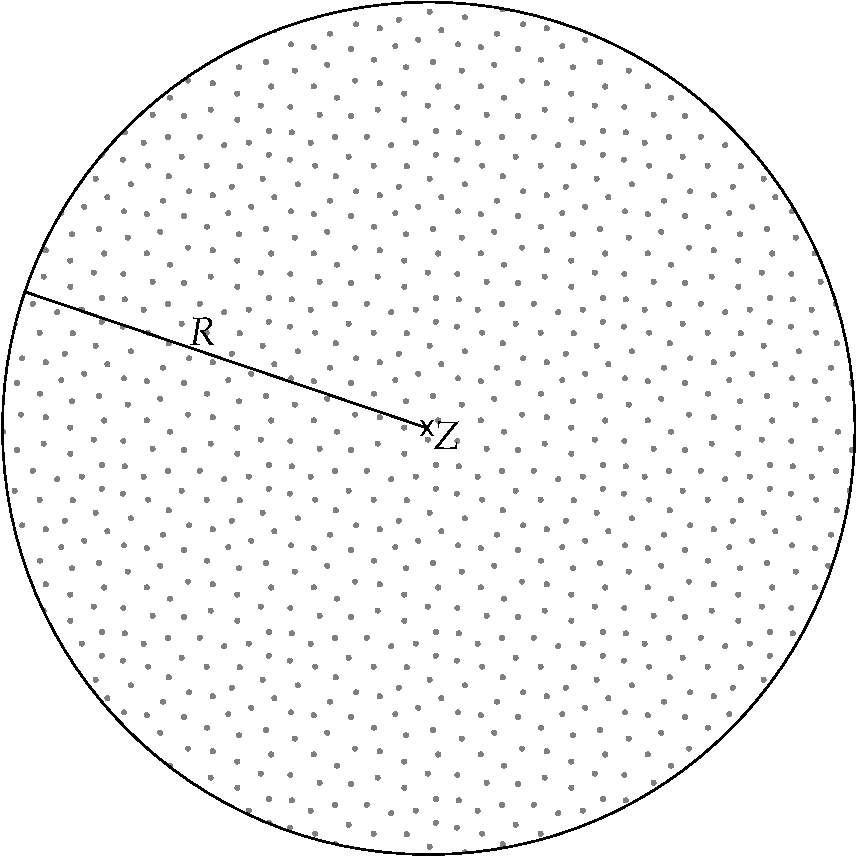
\includegraphics[height=0.7\textheight]{Kopplung_2_Geometrie_2}}
            \only<3>{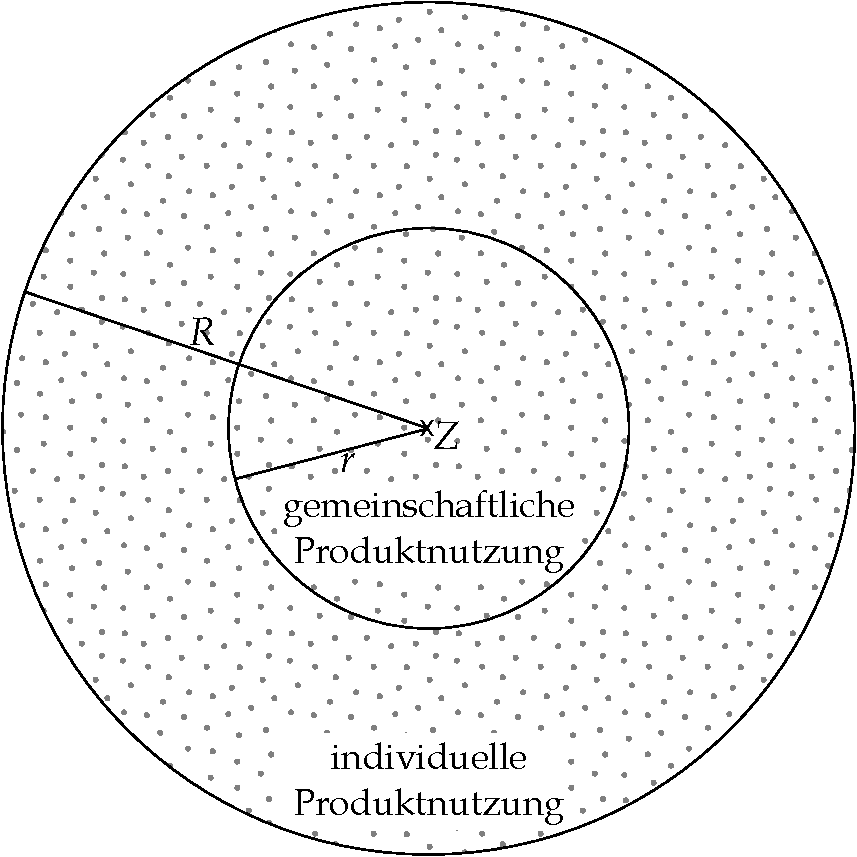
\includegraphics[height=0.7\textheight]{Kopplung_2_Geometrie_3}}
            \only<4>{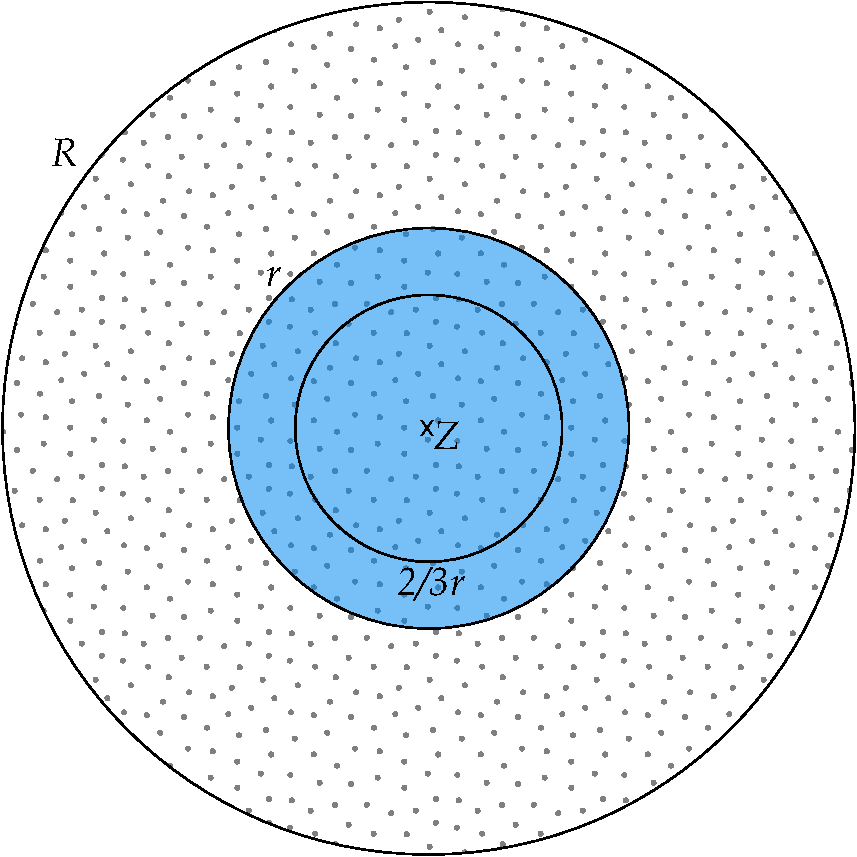
\includegraphics[height=0.7\textheight]{Kopplung_2_Geometrie_4}}
            \only<5>{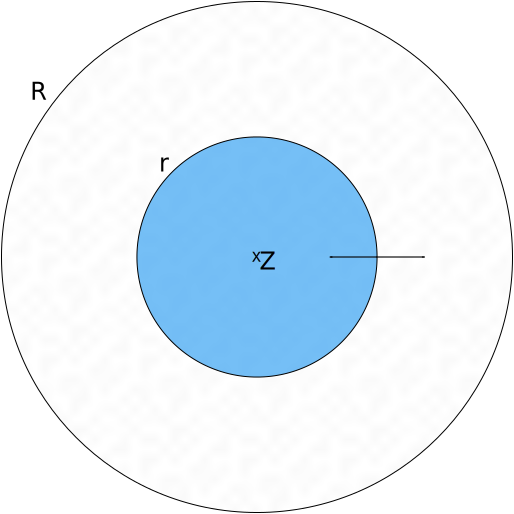
\includegraphics[height=0.7\textheight]{Kopplung_2_Geometrie_5}}
        \end{minipage}
        \begin{minipage}[t]{0.38\textwidth}
            \vspace{0pt} 
            \only<1>{}
            \only<2>{Homogen verteilte Personen-Standorte}
            \only<3>{
                Zwei Teilnutzungssysteme:
                \begin{itemize}
                    \item gemeinschaftliches Nutzungssystem mit $h^\text{gem}$
                    \item individuelles Nutzungssystem mit $h^\text{ind}$
                \end{itemize}
                Es gilt:
                $$h^\text{gem} > h^\text{gem} $$
            }
            \only<4>{
                \begin{itemize}
                \item Individuelles Nutzungssystem: keine Transporte\\
                    $\Rightarrow d^\text{ind} = 0$
                \item Gemeinschaftliches Nutzungssystem: Transporte zwischen
                    Zentrum $Z$ und Personen-Standorten\\
                    $\Rightarrow d^\text{gem} = \frac{2}{3}r$
                \end{itemize}
            }
            \only<5>{
                Variation: \emph{Radius} des gemeinschaftlichen Nutzungssystems
                \begin{itemize}
                    \item Je größer das System, desto mehr Produkte
                        werden eingespart.
                    \item Je größer das System, desto mehr
                        zusätzliche Transporte.
                \end{itemize}
            }
        \end{minipage}
    \end{frame}


    \begin{frame}{Modellbeschreibung}
        \begin{itemize}
            \item MIPS-Gleichung:
                $$\text{MIPS}(r) = \frac{I_P + I_\Theta + I_\text{fix}^{h,d}}{S_D}$$

            \item Transportbezogene Material-Inputs:
                $$I_\Theta \propto S_D^\text{gem} \cdot d^\text{gem} \propto r^2 \cdot r
                = r^3$$

            \item Produktbezogene Material-Inputs:
                $$ I_P \propto P \propto r^2 \cdot \left(
                \frac{q^\text{gem}}{h^\text{gem}} - \frac{q^\text{ind}}{h^\text{ind}}
                \right) + c_1 \qquad (c_1 \dots \text{Konstante})$$
        \end{itemize}
    \end{frame}

    \begin{frame}{Modellanalyse}
       	\begin{block}{Modell: Nutzungsintensivierung und zusätzliche Transporte}<1->
       		$$\text{MIPS}(r) = c_2 \cdot r^2 \cdot \left( \frac{q^\text{gem}}{h^\text{gem}} - \frac{q^\text{ind}}{h^\text{ind}} \right) + c_3 \cdot r^3 + c_4$$
       	\end{block}
    	\only<2-3>{% Created by tikzDevice version 0.8.1 on 2015-07-13 22:50:16
% !TEX encoding = UTF-8 Unicode
\begin{tikzpicture}[x=1pt,y=1pt]
\definecolor{fillColor}{RGB}{255,255,255}
\path[use as bounding box,fill=fillColor,fill opacity=0.00] (0,0) rectangle (317.99,115.63);
\begin{scope}
\path[clip] ( 14.40, 27.00) rectangle (149.99,111.13);
\definecolor{drawColor}{RGB}{0,0,0}

\path[draw=drawColor,line width= 0.4pt,line join=round,line cap=round] ( 19.42, 38.77) --
	( 19.55, 38.77) --
	( 19.67, 38.77) --
	( 19.80, 38.77) --
	( 19.92, 38.77) --
	( 20.05, 38.77) --
	( 20.18, 38.77) --
	( 20.30, 38.77) --
	( 20.43, 38.77) --
	( 20.55, 38.77) --
	( 20.68, 38.77) --
	( 20.80, 38.77) --
	( 20.93, 38.77) --
	( 21.06, 38.77) --
	( 21.18, 38.77) --
	( 21.31, 38.77) --
	( 21.43, 38.77) --
	( 21.56, 38.77) --
	( 21.68, 38.77) --
	( 21.81, 38.77) --
	( 21.94, 38.77) --
	( 22.06, 38.77) --
	( 22.19, 38.77) --
	( 22.31, 38.77) --
	( 22.44, 38.77) --
	( 22.56, 38.77) --
	( 22.69, 38.77) --
	( 22.82, 38.77) --
	( 22.94, 38.77) --
	( 23.07, 38.77) --
	( 23.19, 38.77) --
	( 23.32, 38.77) --
	( 23.44, 38.77) --
	( 23.57, 38.77) --
	( 23.69, 38.77) --
	( 23.82, 38.77) --
	( 23.95, 38.77) --
	( 24.07, 38.78) --
	( 24.20, 38.78) --
	( 24.32, 38.78) --
	( 24.45, 38.78) --
	( 24.57, 38.78) --
	( 24.70, 38.78) --
	( 24.83, 38.78) --
	( 24.95, 38.78) --
	( 25.08, 38.78) --
	( 25.20, 38.78) --
	( 25.33, 38.78) --
	( 25.45, 38.78) --
	( 25.58, 38.78) --
	( 25.71, 38.78) --
	( 25.83, 38.78) --
	( 25.96, 38.78) --
	( 26.08, 38.78) --
	( 26.21, 38.78) --
	( 26.33, 38.78) --
	( 26.46, 38.78) --
	( 26.59, 38.78) --
	( 26.71, 38.79) --
	( 26.84, 38.79) --
	( 26.96, 38.79) --
	( 27.09, 38.79) --
	( 27.21, 38.79) --
	( 27.34, 38.79) --
	( 27.47, 38.79) --
	( 27.59, 38.79) --
	( 27.72, 38.79) --
	( 27.84, 38.79) --
	( 27.97, 38.79) --
	( 28.09, 38.79) --
	( 28.22, 38.80) --
	( 28.34, 38.80) --
	( 28.47, 38.80) --
	( 28.60, 38.80) --
	( 28.72, 38.80) --
	( 28.85, 38.80) --
	( 28.97, 38.80) --
	( 29.10, 38.80) --
	( 29.22, 38.80) --
	( 29.35, 38.81) --
	( 29.48, 38.81) --
	( 29.60, 38.81) --
	( 29.73, 38.81) --
	( 29.85, 38.81) --
	( 29.98, 38.81) --
	( 30.10, 38.81) --
	( 30.23, 38.82) --
	( 30.36, 38.82) --
	( 30.48, 38.82) --
	( 30.61, 38.82) --
	( 30.73, 38.82) --
	( 30.86, 38.82) --
	( 30.98, 38.83) --
	( 31.11, 38.83) --
	( 31.24, 38.83) --
	( 31.36, 38.83) --
	( 31.49, 38.83) --
	( 31.61, 38.83) --
	( 31.74, 38.84) --
	( 31.86, 38.84) --
	( 31.99, 38.84) --
	( 32.12, 38.84) --
	( 32.24, 38.85) --
	( 32.37, 38.85) --
	( 32.49, 38.85) --
	( 32.62, 38.85) --
	( 32.74, 38.85) --
	( 32.87, 38.86) --
	( 32.99, 38.86) --
	( 33.12, 38.86) --
	( 33.25, 38.86) --
	( 33.37, 38.87) --
	( 33.50, 38.87) --
	( 33.62, 38.87) --
	( 33.75, 38.87) --
	( 33.87, 38.88) --
	( 34.00, 38.88) --
	( 34.13, 38.88) --
	( 34.25, 38.89) --
	( 34.38, 38.89) --
	( 34.50, 38.89) --
	( 34.63, 38.89) --
	( 34.75, 38.90) --
	( 34.88, 38.90) --
	( 35.01, 38.90) --
	( 35.13, 38.91) --
	( 35.26, 38.91) --
	( 35.38, 38.91) --
	( 35.51, 38.92) --
	( 35.63, 38.92) --
	( 35.76, 38.92) --
	( 35.89, 38.93) --
	( 36.01, 38.93) --
	( 36.14, 38.93) --
	( 36.26, 38.94) --
	( 36.39, 38.94) --
	( 36.51, 38.95) --
	( 36.64, 38.95) --
	( 36.77, 38.95) --
	( 36.89, 38.96) --
	( 37.02, 38.96) --
	( 37.14, 38.97) --
	( 37.27, 38.97) --
	( 37.39, 38.97) --
	( 37.52, 38.98) --
	( 37.64, 38.98) --
	( 37.77, 38.99) --
	( 37.90, 38.99) --
	( 38.02, 39.00) --
	( 38.15, 39.00) --
	( 38.27, 39.01) --
	( 38.40, 39.01) --
	( 38.52, 39.02) --
	( 38.65, 39.02) --
	( 38.78, 39.03) --
	( 38.90, 39.03) --
	( 39.03, 39.04) --
	( 39.15, 39.04) --
	( 39.28, 39.05) --
	( 39.40, 39.05) --
	( 39.53, 39.06) --
	( 39.66, 39.06) --
	( 39.78, 39.07) --
	( 39.91, 39.07) --
	( 40.03, 39.08) --
	( 40.16, 39.08) --
	( 40.28, 39.09) --
	( 40.41, 39.10) --
	( 40.54, 39.10) --
	( 40.66, 39.11) --
	( 40.79, 39.11) --
	( 40.91, 39.12) --
	( 41.04, 39.12) --
	( 41.16, 39.13) --
	( 41.29, 39.14) --
	( 41.42, 39.14) --
	( 41.54, 39.15) --
	( 41.67, 39.16) --
	( 41.79, 39.16) --
	( 41.92, 39.17) --
	( 42.04, 39.18) --
	( 42.17, 39.18) --
	( 42.29, 39.19) --
	( 42.42, 39.20) --
	( 42.55, 39.20) --
	( 42.67, 39.21) --
	( 42.80, 39.22) --
	( 42.92, 39.23) --
	( 43.05, 39.23) --
	( 43.17, 39.24) --
	( 43.30, 39.25) --
	( 43.43, 39.26) --
	( 43.55, 39.26) --
	( 43.68, 39.27) --
	( 43.80, 39.28) --
	( 43.93, 39.29) --
	( 44.05, 39.29) --
	( 44.18, 39.30) --
	( 44.31, 39.31) --
	( 44.43, 39.32) --
	( 44.56, 39.33) --
	( 44.68, 39.34) --
	( 44.81, 39.34) --
	( 44.93, 39.35) --
	( 45.06, 39.36) --
	( 45.19, 39.37) --
	( 45.31, 39.38) --
	( 45.44, 39.39) --
	( 45.56, 39.40) --
	( 45.69, 39.41) --
	( 45.81, 39.41) --
	( 45.94, 39.42) --
	( 46.07, 39.43) --
	( 46.19, 39.44) --
	( 46.32, 39.45) --
	( 46.44, 39.46) --
	( 46.57, 39.47) --
	( 46.69, 39.48) --
	( 46.82, 39.49) --
	( 46.94, 39.50) --
	( 47.07, 39.51) --
	( 47.20, 39.52) --
	( 47.32, 39.53) --
	( 47.45, 39.54) --
	( 47.57, 39.55) --
	( 47.70, 39.56) --
	( 47.82, 39.57) --
	( 47.95, 39.58) --
	( 48.08, 39.59) --
	( 48.20, 39.61) --
	( 48.33, 39.62) --
	( 48.45, 39.63) --
	( 48.58, 39.64) --
	( 48.70, 39.65) --
	( 48.83, 39.66) --
	( 48.96, 39.67) --
	( 49.08, 39.68) --
	( 49.21, 39.70) --
	( 49.33, 39.71) --
	( 49.46, 39.72) --
	( 49.58, 39.73) --
	( 49.71, 39.74) --
	( 49.84, 39.76) --
	( 49.96, 39.77) --
	( 50.09, 39.78) --
	( 50.21, 39.79) --
	( 50.34, 39.81) --
	( 50.46, 39.82) --
	( 50.59, 39.83) --
	( 50.72, 39.84) --
	( 50.84, 39.86) --
	( 50.97, 39.87) --
	( 51.09, 39.88) --
	( 51.22, 39.90) --
	( 51.34, 39.91) --
	( 51.47, 39.92) --
	( 51.59, 39.94) --
	( 51.72, 39.95) --
	( 51.85, 39.96) --
	( 51.97, 39.98) --
	( 52.10, 39.99) --
	( 52.22, 40.01) --
	( 52.35, 40.02) --
	( 52.47, 40.03) --
	( 52.60, 40.05) --
	( 52.73, 40.06) --
	( 52.85, 40.08) --
	( 52.98, 40.09) --
	( 53.10, 40.11) --
	( 53.23, 40.12) --
	( 53.35, 40.14) --
	( 53.48, 40.15) --
	( 53.61, 40.17) --
	( 53.73, 40.18) --
	( 53.86, 40.20) --
	( 53.98, 40.22) --
	( 54.11, 40.23) --
	( 54.23, 40.25) --
	( 54.36, 40.26) --
	( 54.49, 40.28) --
	( 54.61, 40.30) --
	( 54.74, 40.31) --
	( 54.86, 40.33) --
	( 54.99, 40.35) --
	( 55.11, 40.36) --
	( 55.24, 40.38) --
	( 55.37, 40.40) --
	( 55.49, 40.41) --
	( 55.62, 40.43) --
	( 55.74, 40.45) --
	( 55.87, 40.47) --
	( 55.99, 40.48) --
	( 56.12, 40.50) --
	( 56.24, 40.52) --
	( 56.37, 40.54) --
	( 56.50, 40.55) --
	( 56.62, 40.57) --
	( 56.75, 40.59) --
	( 56.87, 40.61) --
	( 57.00, 40.63) --
	( 57.12, 40.65) --
	( 57.25, 40.67) --
	( 57.38, 40.68) --
	( 57.50, 40.70) --
	( 57.63, 40.72) --
	( 57.75, 40.74) --
	( 57.88, 40.76) --
	( 58.00, 40.78) --
	( 58.13, 40.80) --
	( 58.26, 40.82) --
	( 58.38, 40.84) --
	( 58.51, 40.86) --
	( 58.63, 40.88) --
	( 58.76, 40.90) --
	( 58.88, 40.92) --
	( 59.01, 40.94) --
	( 59.14, 40.96) --
	( 59.26, 40.98) --
	( 59.39, 41.00) --
	( 59.51, 41.03) --
	( 59.64, 41.05) --
	( 59.76, 41.07) --
	( 59.89, 41.09) --
	( 60.02, 41.11) --
	( 60.14, 41.13) --
	( 60.27, 41.16) --
	( 60.39, 41.18) --
	( 60.52, 41.20) --
	( 60.64, 41.22) --
	( 60.77, 41.24) --
	( 60.89, 41.27) --
	( 61.02, 41.29) --
	( 61.15, 41.31) --
	( 61.27, 41.34) --
	( 61.40, 41.36) --
	( 61.52, 41.38) --
	( 61.65, 41.41) --
	( 61.77, 41.43) --
	( 61.90, 41.45) --
	( 62.03, 41.48) --
	( 62.15, 41.50) --
	( 62.28, 41.53) --
	( 62.40, 41.55) --
	( 62.53, 41.57) --
	( 62.65, 41.60) --
	( 62.78, 41.62) --
	( 62.91, 41.65) --
	( 63.03, 41.67) --
	( 63.16, 41.70) --
	( 63.28, 41.72) --
	( 63.41, 41.75) --
	( 63.53, 41.77) --
	( 63.66, 41.80) --
	( 63.79, 41.83) --
	( 63.91, 41.85) --
	( 64.04, 41.88) --
	( 64.16, 41.91) --
	( 64.29, 41.93) --
	( 64.41, 41.96) --
	( 64.54, 41.99) --
	( 64.67, 42.01) --
	( 64.79, 42.04) --
	( 64.92, 42.07) --
	( 65.04, 42.09) --
	( 65.17, 42.12) --
	( 65.29, 42.15) --
	( 65.42, 42.18) --
	( 65.54, 42.20) --
	( 65.67, 42.23) --
	( 65.80, 42.26) --
	( 65.92, 42.29) --
	( 66.05, 42.32) --
	( 66.17, 42.35) --
	( 66.30, 42.38) --
	( 66.42, 42.40) --
	( 66.55, 42.43) --
	( 66.68, 42.46) --
	( 66.80, 42.49) --
	( 66.93, 42.52) --
	( 67.05, 42.55) --
	( 67.18, 42.58) --
	( 67.30, 42.61) --
	( 67.43, 42.64) --
	( 67.56, 42.67) --
	( 67.68, 42.70) --
	( 67.81, 42.73) --
	( 67.93, 42.77) --
	( 68.06, 42.80) --
	( 68.18, 42.83) --
	( 68.31, 42.86) --
	( 68.44, 42.89) --
	( 68.56, 42.92) --
	( 68.69, 42.96) --
	( 68.81, 42.99) --
	( 68.94, 43.02) --
	( 69.06, 43.05) --
	( 69.19, 43.08) --
	( 69.32, 43.12) --
	( 69.44, 43.15) --
	( 69.57, 43.18) --
	( 69.69, 43.22) --
	( 69.82, 43.25) --
	( 69.94, 43.28) --
	( 70.07, 43.32) --
	( 70.19, 43.35) --
	( 70.32, 43.39) --
	( 70.45, 43.42) --
	( 70.57, 43.45) --
	( 70.70, 43.49) --
	( 70.82, 43.52) --
	( 70.95, 43.56) --
	( 71.07, 43.59) --
	( 71.20, 43.63) --
	( 71.33, 43.66) --
	( 71.45, 43.70) --
	( 71.58, 43.74) --
	( 71.70, 43.77) --
	( 71.83, 43.81) --
	( 71.95, 43.84) --
	( 72.08, 43.88) --
	( 72.21, 43.92) --
	( 72.33, 43.95) --
	( 72.46, 43.99) --
	( 72.58, 44.03) --
	( 72.71, 44.07) --
	( 72.83, 44.10) --
	( 72.96, 44.14) --
	( 73.09, 44.18) --
	( 73.21, 44.22) --
	( 73.34, 44.26) --
	( 73.46, 44.29) --
	( 73.59, 44.33) --
	( 73.71, 44.37) --
	( 73.84, 44.41) --
	( 73.97, 44.45) --
	( 74.09, 44.49) --
	( 74.22, 44.53) --
	( 74.34, 44.57) --
	( 74.47, 44.61) --
	( 74.59, 44.65) --
	( 74.72, 44.69) --
	( 74.84, 44.73) --
	( 74.97, 44.77) --
	( 75.10, 44.81) --
	( 75.22, 44.85) --
	( 75.35, 44.89) --
	( 75.47, 44.93) --
	( 75.60, 44.97) --
	( 75.72, 45.02) --
	( 75.85, 45.06) --
	( 75.98, 45.10) --
	( 76.10, 45.14) --
	( 76.23, 45.19) --
	( 76.35, 45.23) --
	( 76.48, 45.27) --
	( 76.60, 45.31) --
	( 76.73, 45.36) --
	( 76.86, 45.40) --
	( 76.98, 45.44) --
	( 77.11, 45.49) --
	( 77.23, 45.53) --
	( 77.36, 45.58) --
	( 77.48, 45.62) --
	( 77.61, 45.66) --
	( 77.74, 45.71) --
	( 77.86, 45.75) --
	( 77.99, 45.80) --
	( 78.11, 45.85) --
	( 78.24, 45.89) --
	( 78.36, 45.94) --
	( 78.49, 45.98) --
	( 78.62, 46.03) --
	( 78.74, 46.07) --
	( 78.87, 46.12) --
	( 78.99, 46.17) --
	( 79.12, 46.21) --
	( 79.24, 46.26) --
	( 79.37, 46.31) --
	( 79.49, 46.36) --
	( 79.62, 46.40) --
	( 79.75, 46.45) --
	( 79.87, 46.50) --
	( 80.00, 46.55) --
	( 80.12, 46.60) --
	( 80.25, 46.65) --
	( 80.37, 46.69) --
	( 80.50, 46.74) --
	( 80.63, 46.79) --
	( 80.75, 46.84) --
	( 80.88, 46.89) --
	( 81.00, 46.94) --
	( 81.13, 46.99) --
	( 81.25, 47.04) --
	( 81.38, 47.09) --
	( 81.51, 47.14) --
	( 81.63, 47.20) --
	( 81.76, 47.25) --
	( 81.88, 47.30) --
	( 82.01, 47.35) --
	( 82.13, 47.40) --
	( 82.26, 47.45) --
	( 82.39, 47.51) --
	( 82.51, 47.56) --
	( 82.64, 47.61) --
	( 82.76, 47.66) --
	( 82.89, 47.72) --
	( 83.01, 47.77) --
	( 83.14, 47.82) --
	( 83.27, 47.88) --
	( 83.39, 47.93) --
	( 83.52, 47.98) --
	( 83.64, 48.04) --
	( 83.77, 48.09) --
	( 83.89, 48.15) --
	( 84.02, 48.20) --
	( 84.14, 48.26) --
	( 84.27, 48.31) --
	( 84.40, 48.37) --
	( 84.52, 48.42) --
	( 84.65, 48.48) --
	( 84.77, 48.54) --
	( 84.90, 48.59) --
	( 85.02, 48.65) --
	( 85.15, 48.71) --
	( 85.28, 48.76) --
	( 85.40, 48.82) --
	( 85.53, 48.88) --
	( 85.65, 48.94) --
	( 85.78, 48.99) --
	( 85.90, 49.05) --
	( 86.03, 49.11) --
	( 86.16, 49.17) --
	( 86.28, 49.23) --
	( 86.41, 49.29) --
	( 86.53, 49.35) --
	( 86.66, 49.41) --
	( 86.78, 49.47) --
	( 86.91, 49.53) --
	( 87.04, 49.59) --
	( 87.16, 49.65) --
	( 87.29, 49.71) --
	( 87.41, 49.77) --
	( 87.54, 49.83) --
	( 87.66, 49.89) --
	( 87.79, 49.95) --
	( 87.92, 50.01) --
	( 88.04, 50.08) --
	( 88.17, 50.14) --
	( 88.29, 50.20) --
	( 88.42, 50.26) --
	( 88.54, 50.33) --
	( 88.67, 50.39) --
	( 88.79, 50.45) --
	( 88.92, 50.52) --
	( 89.05, 50.58) --
	( 89.17, 50.64) --
	( 89.30, 50.71) --
	( 89.42, 50.77) --
	( 89.55, 50.84) --
	( 89.67, 50.90) --
	( 89.80, 50.97) --
	( 89.93, 51.03) --
	( 90.05, 51.10) --
	( 90.18, 51.17) --
	( 90.30, 51.23) --
	( 90.43, 51.30) --
	( 90.55, 51.36) --
	( 90.68, 51.43) --
	( 90.81, 51.50) --
	( 90.93, 51.57) --
	( 91.06, 51.63) --
	( 91.18, 51.70) --
	( 91.31, 51.77) --
	( 91.43, 51.84) --
	( 91.56, 51.91) --
	( 91.69, 51.98) --
	( 91.81, 52.04) --
	( 91.94, 52.11) --
	( 92.06, 52.18) --
	( 92.19, 52.25) --
	( 92.31, 52.32) --
	( 92.44, 52.39) --
	( 92.57, 52.46) --
	( 92.69, 52.53) --
	( 92.82, 52.60) --
	( 92.94, 52.68) --
	( 93.07, 52.75) --
	( 93.19, 52.82) --
	( 93.32, 52.89) --
	( 93.44, 52.96) --
	( 93.57, 53.04) --
	( 93.70, 53.11) --
	( 93.82, 53.18) --
	( 93.95, 53.25) --
	( 94.07, 53.33) --
	( 94.20, 53.40) --
	( 94.32, 53.48) --
	( 94.45, 53.55) --
	( 94.58, 53.62) --
	( 94.70, 53.70) --
	( 94.83, 53.77) --
	( 94.95, 53.85) --
	( 95.08, 53.92) --
	( 95.20, 54.00) --
	( 95.33, 54.08) --
	( 95.46, 54.15) --
	( 95.58, 54.23) --
	( 95.71, 54.30) --
	( 95.83, 54.38) --
	( 95.96, 54.46) --
	( 96.08, 54.54) --
	( 96.21, 54.61) --
	( 96.34, 54.69) --
	( 96.46, 54.77) --
	( 96.59, 54.85) --
	( 96.71, 54.93) --
	( 96.84, 55.01) --
	( 96.96, 55.08) --
	( 97.09, 55.16) --
	( 97.22, 55.24) --
	( 97.34, 55.32) --
	( 97.47, 55.40) --
	( 97.59, 55.48) --
	( 97.72, 55.57) --
	( 97.84, 55.65) --
	( 97.97, 55.73) --
	( 98.09, 55.81) --
	( 98.22, 55.89) --
	( 98.35, 55.97) --
	( 98.47, 56.06) --
	( 98.60, 56.14) --
	( 98.72, 56.22) --
	( 98.85, 56.30) --
	( 98.97, 56.39) --
	( 99.10, 56.47) --
	( 99.23, 56.55) --
	( 99.35, 56.64) --
	( 99.48, 56.72) --
	( 99.60, 56.81) --
	( 99.73, 56.89) --
	( 99.85, 56.98) --
	( 99.98, 57.06) --
	(100.11, 57.15) --
	(100.23, 57.24) --
	(100.36, 57.32) --
	(100.48, 57.41) --
	(100.61, 57.50) --
	(100.73, 57.58) --
	(100.86, 57.67) --
	(100.99, 57.76) --
	(101.11, 57.84) --
	(101.24, 57.93) --
	(101.36, 58.02) --
	(101.49, 58.11) --
	(101.61, 58.20) --
	(101.74, 58.29) --
	(101.87, 58.38) --
	(101.99, 58.47) --
	(102.12, 58.56) --
	(102.24, 58.65) --
	(102.37, 58.74) --
	(102.49, 58.83) --
	(102.62, 58.92) --
	(102.74, 59.01) --
	(102.87, 59.10) --
	(103.00, 59.20) --
	(103.12, 59.29) --
	(103.25, 59.38) --
	(103.37, 59.47) --
	(103.50, 59.57) --
	(103.62, 59.66) --
	(103.75, 59.75) --
	(103.88, 59.85) --
	(104.00, 59.94) --
	(104.13, 60.04) --
	(104.25, 60.13) --
	(104.38, 60.23) --
	(104.50, 60.32) --
	(104.63, 60.42) --
	(104.76, 60.51) --
	(104.88, 60.61) --
	(105.01, 60.71) --
	(105.13, 60.80) --
	(105.26, 60.90) --
	(105.38, 61.00) --
	(105.51, 61.09) --
	(105.64, 61.19) --
	(105.76, 61.29) --
	(105.89, 61.39) --
	(106.01, 61.49) --
	(106.14, 61.59) --
	(106.26, 61.69) --
	(106.39, 61.79) --
	(106.52, 61.89) --
	(106.64, 61.99) --
	(106.77, 62.09) --
	(106.89, 62.19) --
	(107.02, 62.29) --
	(107.14, 62.39) --
	(107.27, 62.49) --
	(107.39, 62.59) --
	(107.52, 62.70) --
	(107.65, 62.80) --
	(107.77, 62.90) --
	(107.90, 63.00) --
	(108.02, 63.11) --
	(108.15, 63.21) --
	(108.27, 63.32) --
	(108.40, 63.42) --
	(108.53, 63.52) --
	(108.65, 63.63) --
	(108.78, 63.73) --
	(108.90, 63.84) --
	(109.03, 63.95) --
	(109.15, 64.05) --
	(109.28, 64.16) --
	(109.41, 64.26) --
	(109.53, 64.37) --
	(109.66, 64.48) --
	(109.78, 64.59) --
	(109.91, 64.69) --
	(110.03, 64.80) --
	(110.16, 64.91) --
	(110.29, 65.02) --
	(110.41, 65.13) --
	(110.54, 65.24) --
	(110.66, 65.35) --
	(110.79, 65.46) --
	(110.91, 65.57) --
	(111.04, 65.68) --
	(111.17, 65.79) --
	(111.29, 65.90) --
	(111.42, 66.01) --
	(111.54, 66.12) --
	(111.67, 66.24) --
	(111.79, 66.35) --
	(111.92, 66.46) --
	(112.04, 66.57) --
	(112.17, 66.69) --
	(112.30, 66.80) --
	(112.42, 66.92) --
	(112.55, 67.03) --
	(112.67, 67.14) --
	(112.80, 67.26) --
	(112.92, 67.37) --
	(113.05, 67.49) --
	(113.18, 67.61) --
	(113.30, 67.72) --
	(113.43, 67.84) --
	(113.55, 67.95) --
	(113.68, 68.07) --
	(113.80, 68.19) --
	(113.93, 68.31) --
	(114.06, 68.42) --
	(114.18, 68.54) --
	(114.31, 68.66) --
	(114.43, 68.78) --
	(114.56, 68.90) --
	(114.68, 69.02) --
	(114.81, 69.14) --
	(114.94, 69.26) --
	(115.06, 69.38) --
	(115.19, 69.50) --
	(115.31, 69.62) --
	(115.44, 69.74) --
	(115.56, 69.87) --
	(115.69, 69.99) --
	(115.82, 70.11) --
	(115.94, 70.23) --
	(116.07, 70.36) --
	(116.19, 70.48) --
	(116.32, 70.60) --
	(116.44, 70.73) --
	(116.57, 70.85) --
	(116.69, 70.98) --
	(116.82, 71.10) --
	(116.95, 71.23) --
	(117.07, 71.35) --
	(117.20, 71.48) --
	(117.32, 71.60) --
	(117.45, 71.73) --
	(117.57, 71.86) --
	(117.70, 71.98) --
	(117.83, 72.11) --
	(117.95, 72.24) --
	(118.08, 72.37) --
	(118.20, 72.50) --
	(118.33, 72.63) --
	(118.45, 72.75) --
	(118.58, 72.88) --
	(118.71, 73.01) --
	(118.83, 73.14) --
	(118.96, 73.28) --
	(119.08, 73.41) --
	(119.21, 73.54) --
	(119.33, 73.67) --
	(119.46, 73.80) --
	(119.59, 73.93) --
	(119.71, 74.07) --
	(119.84, 74.20) --
	(119.96, 74.33) --
	(120.09, 74.46) --
	(120.21, 74.60) --
	(120.34, 74.73) --
	(120.47, 74.87) --
	(120.59, 75.00) --
	(120.72, 75.14) --
	(120.84, 75.27) --
	(120.97, 75.41) --
	(121.09, 75.54) --
	(121.22, 75.68) --
	(121.34, 75.82) --
	(121.47, 75.96) --
	(121.60, 76.09) --
	(121.72, 76.23) --
	(121.85, 76.37) --
	(121.97, 76.51) --
	(122.10, 76.65) --
	(122.22, 76.79) --
	(122.35, 76.93) --
	(122.48, 77.07) --
	(122.60, 77.21) --
	(122.73, 77.35) --
	(122.85, 77.49) --
	(122.98, 77.63) --
	(123.10, 77.77) --
	(123.23, 77.91) --
	(123.36, 78.05) --
	(123.48, 78.20) --
	(123.61, 78.34) --
	(123.73, 78.48) --
	(123.86, 78.63) --
	(123.98, 78.77) --
	(124.11, 78.92) --
	(124.24, 79.06) --
	(124.36, 79.21) --
	(124.49, 79.35) --
	(124.61, 79.50) --
	(124.74, 79.64) --
	(124.86, 79.79) --
	(124.99, 79.94) --
	(125.12, 80.08) --
	(125.24, 80.23) --
	(125.37, 80.38) --
	(125.49, 80.53) --
	(125.62, 80.68) --
	(125.74, 80.82) --
	(125.87, 80.97) --
	(125.99, 81.12) --
	(126.12, 81.27) --
	(126.25, 81.42) --
	(126.37, 81.57) --
	(126.50, 81.73) --
	(126.62, 81.88) --
	(126.75, 82.03) --
	(126.87, 82.18) --
	(127.00, 82.33) --
	(127.13, 82.49) --
	(127.25, 82.64) --
	(127.38, 82.79) --
	(127.50, 82.95) --
	(127.63, 83.10) --
	(127.75, 83.26) --
	(127.88, 83.41) --
	(128.01, 83.57) --
	(128.13, 83.72) --
	(128.26, 83.88) --
	(128.38, 84.03) --
	(128.51, 84.19) --
	(128.63, 84.35) --
	(128.76, 84.51) --
	(128.89, 84.66) --
	(129.01, 84.82) --
	(129.14, 84.98) --
	(129.26, 85.14) --
	(129.39, 85.30) --
	(129.51, 85.46) --
	(129.64, 85.62) --
	(129.77, 85.78) --
	(129.89, 85.94) --
	(130.02, 86.10) --
	(130.14, 86.26) --
	(130.27, 86.42) --
	(130.39, 86.59) --
	(130.52, 86.75) --
	(130.64, 86.91) --
	(130.77, 87.08) --
	(130.90, 87.24) --
	(131.02, 87.40) --
	(131.15, 87.57) --
	(131.27, 87.73) --
	(131.40, 87.90) --
	(131.52, 88.06) --
	(131.65, 88.23) --
	(131.78, 88.40) --
	(131.90, 88.56) --
	(132.03, 88.73) --
	(132.15, 88.90) --
	(132.28, 89.07) --
	(132.40, 89.23) --
	(132.53, 89.40) --
	(132.66, 89.57) --
	(132.78, 89.74) --
	(132.91, 89.91) --
	(133.03, 90.08) --
	(133.16, 90.25) --
	(133.28, 90.42) --
	(133.41, 90.59) --
	(133.54, 90.76) --
	(133.66, 90.94) --
	(133.79, 91.11) --
	(133.91, 91.28) --
	(134.04, 91.45) --
	(134.16, 91.63) --
	(134.29, 91.80) --
	(134.42, 91.98) --
	(134.54, 92.15) --
	(134.67, 92.33) --
	(134.79, 92.50) --
	(134.92, 92.68) --
	(135.04, 92.85) --
	(135.17, 93.03) --
	(135.29, 93.21) --
	(135.42, 93.38) --
	(135.55, 93.56) --
	(135.67, 93.74) --
	(135.80, 93.92) --
	(135.92, 94.10) --
	(136.05, 94.28) --
	(136.17, 94.46) --
	(136.30, 94.64) --
	(136.43, 94.82) --
	(136.55, 95.00) --
	(136.68, 95.18) --
	(136.80, 95.36) --
	(136.93, 95.54) --
	(137.05, 95.72) --
	(137.18, 95.91) --
	(137.31, 96.09) --
	(137.43, 96.27) --
	(137.56, 96.46) --
	(137.68, 96.64) --
	(137.81, 96.83) --
	(137.93, 97.01) --
	(138.06, 97.20) --
	(138.19, 97.38) --
	(138.31, 97.57) --
	(138.44, 97.76) --
	(138.56, 97.94) --
	(138.69, 98.13) --
	(138.81, 98.32) --
	(138.94, 98.51) --
	(139.07, 98.70) --
	(139.19, 98.88) --
	(139.32, 99.07) --
	(139.44, 99.26) --
	(139.57, 99.45) --
	(139.69, 99.64) --
	(139.82, 99.84) --
	(139.94,100.03) --
	(140.07,100.22) --
	(140.20,100.41) --
	(140.32,100.60) --
	(140.45,100.80) --
	(140.57,100.99) --
	(140.70,101.18) --
	(140.82,101.38) --
	(140.95,101.57) --
	(141.08,101.77) --
	(141.20,101.96) --
	(141.33,102.16) --
	(141.45,102.36) --
	(141.58,102.55) --
	(141.70,102.75) --
	(141.83,102.95) --
	(141.96,103.14) --
	(142.08,103.34) --
	(142.21,103.54) --
	(142.33,103.74) --
	(142.46,103.94) --
	(142.58,104.14) --
	(142.71,104.34) --
	(142.84,104.54) --
	(142.96,104.74) --
	(143.09,104.94) --
	(143.21,105.15) --
	(143.34,105.35) --
	(143.46,105.55) --
	(143.59,105.75) --
	(143.72,105.96) --
	(143.84,106.16) --
	(143.97,106.37) --
	(144.09,106.57) --
	(144.22,106.78) --
	(144.34,106.98) --
	(144.47,107.19) --
	(144.59,107.39) --
	(144.72,107.60) --
	(144.85,107.81) --
	(144.97,108.02);
\end{scope}
\begin{scope}
\path[clip] (  0.00,  0.00) rectangle (317.99,115.63);
\definecolor{drawColor}{RGB}{0,0,0}

\path[draw=drawColor,line width= 0.4pt,line join=round,line cap=round] ( 14.40, 27.00) --
	(149.99, 27.00) --
	(149.99,111.13) --
	( 14.40,111.13) --
	( 14.40, 27.00);
\end{scope}
\begin{scope}
\path[clip] (  0.00,  0.00) rectangle (317.99,115.63);
\definecolor{drawColor}{RGB}{0,0,0}

\node[text=drawColor,anchor=base,inner sep=0pt, outer sep=0pt, scale=  0.75] at ( 82.20,  4.50) {Radius $r$};

\node[text=drawColor,rotate= 90.00,anchor=base,inner sep=0pt, outer sep=0pt, scale=  0.75] at (  6.30, 69.07) {$\text{MIPS}(r)$};
\end{scope}
\begin{scope}
\path[clip] (173.39, 27.00) rectangle (308.99,111.13);
\definecolor{drawColor}{RGB}{0,0,0}

\path[draw=drawColor,line width= 0.4pt,line join=round,line cap=round] (178.42, 56.08) --
	(178.54, 56.08) --
	(178.67, 56.08) --
	(178.79, 56.08) --
	(178.92, 56.08) --
	(179.04, 56.08) --
	(179.17, 56.08) --
	(179.30, 56.08) --
	(179.42, 56.07) --
	(179.55, 56.07) --
	(179.67, 56.07) --
	(179.80, 56.06) --
	(179.92, 56.06) --
	(180.05, 56.06) --
	(180.18, 56.05) --
	(180.30, 56.05) --
	(180.43, 56.04) --
	(180.55, 56.04) --
	(180.68, 56.03) --
	(180.80, 56.03) --
	(180.93, 56.02) --
	(181.06, 56.02) --
	(181.18, 56.01) --
	(181.31, 56.00) --
	(181.43, 56.00) --
	(181.56, 55.99) --
	(181.68, 55.98) --
	(181.81, 55.97) --
	(181.93, 55.96) --
	(182.06, 55.96) --
	(182.19, 55.95) --
	(182.31, 55.94) --
	(182.44, 55.93) --
	(182.56, 55.92) --
	(182.69, 55.91) --
	(182.81, 55.90) --
	(182.94, 55.89) --
	(183.07, 55.88) --
	(183.19, 55.87) --
	(183.32, 55.86) --
	(183.44, 55.85) --
	(183.57, 55.83) --
	(183.69, 55.82) --
	(183.82, 55.81) --
	(183.95, 55.80) --
	(184.07, 55.79) --
	(184.20, 55.77) --
	(184.32, 55.76) --
	(184.45, 55.75) --
	(184.57, 55.73) --
	(184.70, 55.72) --
	(184.83, 55.70) --
	(184.95, 55.69) --
	(185.08, 55.68) --
	(185.20, 55.66) --
	(185.33, 55.65) --
	(185.45, 55.63) --
	(185.58, 55.61) --
	(185.71, 55.60) --
	(185.83, 55.58) --
	(185.96, 55.57) --
	(186.08, 55.55) --
	(186.21, 55.53) --
	(186.33, 55.52) --
	(186.46, 55.50) --
	(186.58, 55.48) --
	(186.71, 55.46) --
	(186.84, 55.44) --
	(186.96, 55.43) --
	(187.09, 55.41) --
	(187.21, 55.39) --
	(187.34, 55.37) --
	(187.46, 55.35) --
	(187.59, 55.33) --
	(187.72, 55.31) --
	(187.84, 55.29) --
	(187.97, 55.27) --
	(188.09, 55.25) --
	(188.22, 55.23) --
	(188.34, 55.21) --
	(188.47, 55.19) --
	(188.60, 55.17) --
	(188.72, 55.15) --
	(188.85, 55.13) --
	(188.97, 55.10) --
	(189.10, 55.08) --
	(189.22, 55.06) --
	(189.35, 55.04) --
	(189.48, 55.02) --
	(189.60, 54.99) --
	(189.73, 54.97) --
	(189.85, 54.95) --
	(189.98, 54.92) --
	(190.10, 54.90) --
	(190.23, 54.88) --
	(190.36, 54.85) --
	(190.48, 54.83) --
	(190.61, 54.80) --
	(190.73, 54.78) --
	(190.86, 54.75) --
	(190.98, 54.73) --
	(191.11, 54.70) --
	(191.23, 54.68) --
	(191.36, 54.65) --
	(191.49, 54.63) --
	(191.61, 54.60) --
	(191.74, 54.58) --
	(191.86, 54.55) --
	(191.99, 54.52) --
	(192.11, 54.50) --
	(192.24, 54.47) --
	(192.37, 54.44) --
	(192.49, 54.42) --
	(192.62, 54.39) --
	(192.74, 54.36) --
	(192.87, 54.33) --
	(192.99, 54.31) --
	(193.12, 54.28) --
	(193.25, 54.25) --
	(193.37, 54.22) --
	(193.50, 54.19) --
	(193.62, 54.17) --
	(193.75, 54.14) --
	(193.87, 54.11) --
	(194.00, 54.08) --
	(194.13, 54.05) --
	(194.25, 54.02) --
	(194.38, 53.99) --
	(194.50, 53.96) --
	(194.63, 53.93) --
	(194.75, 53.90) --
	(194.88, 53.87) --
	(195.01, 53.84) --
	(195.13, 53.81) --
	(195.26, 53.78) --
	(195.38, 53.75) --
	(195.51, 53.72) --
	(195.63, 53.69) --
	(195.76, 53.66) --
	(195.88, 53.63) --
	(196.01, 53.59) --
	(196.14, 53.56) --
	(196.26, 53.53) --
	(196.39, 53.50) --
	(196.51, 53.47) --
	(196.64, 53.44) --
	(196.76, 53.40) --
	(196.89, 53.37) --
	(197.02, 53.34) --
	(197.14, 53.31) --
	(197.27, 53.27) --
	(197.39, 53.24) --
	(197.52, 53.21) --
	(197.64, 53.17) --
	(197.77, 53.14) --
	(197.90, 53.11) --
	(198.02, 53.07) --
	(198.15, 53.04) --
	(198.27, 53.01) --
	(198.40, 52.97) --
	(198.52, 52.94) --
	(198.65, 52.91) --
	(198.78, 52.87) --
	(198.90, 52.84) --
	(199.03, 52.80) --
	(199.15, 52.77) --
	(199.28, 52.73) --
	(199.40, 52.70) --
	(199.53, 52.66) --
	(199.66, 52.63) --
	(199.78, 52.59) --
	(199.91, 52.56) --
	(200.03, 52.52) --
	(200.16, 52.49) --
	(200.28, 52.45) --
	(200.41, 52.42) --
	(200.53, 52.38) --
	(200.66, 52.35) --
	(200.79, 52.31) --
	(200.91, 52.28) --
	(201.04, 52.24) --
	(201.16, 52.20) --
	(201.29, 52.17) --
	(201.41, 52.13) --
	(201.54, 52.10) --
	(201.67, 52.06) --
	(201.79, 52.02) --
	(201.92, 51.99) --
	(202.04, 51.95) --
	(202.17, 51.91) --
	(202.29, 51.88) --
	(202.42, 51.84) --
	(202.55, 51.80) --
	(202.67, 51.77) --
	(202.80, 51.73) --
	(202.92, 51.69) --
	(203.05, 51.65) --
	(203.17, 51.62) --
	(203.30, 51.58) --
	(203.43, 51.54) --
	(203.55, 51.51) --
	(203.68, 51.47) --
	(203.80, 51.43) --
	(203.93, 51.39) --
	(204.05, 51.35) --
	(204.18, 51.32) --
	(204.31, 51.28) --
	(204.43, 51.24) --
	(204.56, 51.20) --
	(204.68, 51.17) --
	(204.81, 51.13) --
	(204.93, 51.09) --
	(205.06, 51.05) --
	(205.18, 51.01) --
	(205.31, 50.98) --
	(205.44, 50.94) --
	(205.56, 50.90) --
	(205.69, 50.86) --
	(205.81, 50.82) --
	(205.94, 50.78) --
	(206.06, 50.75) --
	(206.19, 50.71) --
	(206.32, 50.67) --
	(206.44, 50.63) --
	(206.57, 50.59) --
	(206.69, 50.55) --
	(206.82, 50.51) --
	(206.94, 50.48) --
	(207.07, 50.44) --
	(207.20, 50.40) --
	(207.32, 50.36) --
	(207.45, 50.32) --
	(207.57, 50.28) --
	(207.70, 50.24) --
	(207.82, 50.20) --
	(207.95, 50.17) --
	(208.08, 50.13) --
	(208.20, 50.09) --
	(208.33, 50.05) --
	(208.45, 50.01) --
	(208.58, 49.97) --
	(208.70, 49.93) --
	(208.83, 49.89) --
	(208.96, 49.85) --
	(209.08, 49.82) --
	(209.21, 49.78) --
	(209.33, 49.74) --
	(209.46, 49.70) --
	(209.58, 49.66) --
	(209.71, 49.62) --
	(209.83, 49.58) --
	(209.96, 49.54) --
	(210.09, 49.50) --
	(210.21, 49.46) --
	(210.34, 49.43) --
	(210.46, 49.39) --
	(210.59, 49.35) --
	(210.71, 49.31) --
	(210.84, 49.27) --
	(210.97, 49.23) --
	(211.09, 49.19) --
	(211.22, 49.15) --
	(211.34, 49.11) --
	(211.47, 49.07) --
	(211.59, 49.04) --
	(211.72, 49.00) --
	(211.85, 48.96) --
	(211.97, 48.92) --
	(212.10, 48.88) --
	(212.22, 48.84) --
	(212.35, 48.80) --
	(212.47, 48.76) --
	(212.60, 48.73) --
	(212.73, 48.69) --
	(212.85, 48.65) --
	(212.98, 48.61) --
	(213.10, 48.57) --
	(213.23, 48.53) --
	(213.35, 48.49) --
	(213.48, 48.46) --
	(213.61, 48.42) --
	(213.73, 48.38) --
	(213.86, 48.34) --
	(213.98, 48.30) --
	(214.11, 48.26) --
	(214.23, 48.23) --
	(214.36, 48.19) --
	(214.48, 48.15) --
	(214.61, 48.11) --
	(214.74, 48.07) --
	(214.86, 48.04) --
	(214.99, 48.00) --
	(215.11, 47.96) --
	(215.24, 47.92) --
	(215.36, 47.88) --
	(215.49, 47.85) --
	(215.62, 47.81) --
	(215.74, 47.77) --
	(215.87, 47.73) --
	(215.99, 47.70) --
	(216.12, 47.66) --
	(216.24, 47.62) --
	(216.37, 47.58) --
	(216.50, 47.55) --
	(216.62, 47.51) --
	(216.75, 47.47) --
	(216.87, 47.43) --
	(217.00, 47.40) --
	(217.12, 47.36) --
	(217.25, 47.32) --
	(217.38, 47.29) --
	(217.50, 47.25) --
	(217.63, 47.21) --
	(217.75, 47.18) --
	(217.88, 47.14) --
	(218.00, 47.10) --
	(218.13, 47.07) --
	(218.26, 47.03) --
	(218.38, 47.00) --
	(218.51, 46.96) --
	(218.63, 46.92) --
	(218.76, 46.89) --
	(218.88, 46.85) --
	(219.01, 46.82) --
	(219.13, 46.78) --
	(219.26, 46.75) --
	(219.39, 46.71) --
	(219.51, 46.68) --
	(219.64, 46.64) --
	(219.76, 46.60) --
	(219.89, 46.57) --
	(220.01, 46.53) --
	(220.14, 46.50) --
	(220.27, 46.47) --
	(220.39, 46.43) --
	(220.52, 46.40) --
	(220.64, 46.36) --
	(220.77, 46.33) --
	(220.89, 46.29) --
	(221.02, 46.26) --
	(221.15, 46.23) --
	(221.27, 46.19) --
	(221.40, 46.16) --
	(221.52, 46.12) --
	(221.65, 46.09) --
	(221.77, 46.06) --
	(221.90, 46.02) --
	(222.03, 45.99) --
	(222.15, 45.96) --
	(222.28, 45.93) --
	(222.40, 45.89) --
	(222.53, 45.86) --
	(222.65, 45.83) --
	(222.78, 45.79) --
	(222.91, 45.76) --
	(223.03, 45.73) --
	(223.16, 45.70) --
	(223.28, 45.67) --
	(223.41, 45.63) --
	(223.53, 45.60) --
	(223.66, 45.57) --
	(223.78, 45.54) --
	(223.91, 45.51) --
	(224.04, 45.48) --
	(224.16, 45.45) --
	(224.29, 45.42) --
	(224.41, 45.39) --
	(224.54, 45.36) --
	(224.66, 45.33) --
	(224.79, 45.29) --
	(224.92, 45.26) --
	(225.04, 45.23) --
	(225.17, 45.21) --
	(225.29, 45.18) --
	(225.42, 45.15) --
	(225.54, 45.12) --
	(225.67, 45.09) --
	(225.80, 45.06) --
	(225.92, 45.03) --
	(226.05, 45.00) --
	(226.17, 44.97) --
	(226.30, 44.94) --
	(226.42, 44.92) --
	(226.55, 44.89) --
	(226.68, 44.86) --
	(226.80, 44.83) --
	(226.93, 44.81) --
	(227.05, 44.78) --
	(227.18, 44.75) --
	(227.30, 44.72) --
	(227.43, 44.70) --
	(227.56, 44.67) --
	(227.68, 44.64) --
	(227.81, 44.62) --
	(227.93, 44.59) --
	(228.06, 44.57) --
	(228.18, 44.54) --
	(228.31, 44.52) --
	(228.43, 44.49) --
	(228.56, 44.46) --
	(228.69, 44.44) --
	(228.81, 44.41) --
	(228.94, 44.39) --
	(229.06, 44.37) --
	(229.19, 44.34) --
	(229.31, 44.32) --
	(229.44, 44.29) --
	(229.57, 44.27) --
	(229.69, 44.25) --
	(229.82, 44.22) --
	(229.94, 44.20) --
	(230.07, 44.18) --
	(230.19, 44.15) --
	(230.32, 44.13) --
	(230.45, 44.11) --
	(230.57, 44.09) --
	(230.70, 44.07) --
	(230.82, 44.04) --
	(230.95, 44.02) --
	(231.07, 44.00) --
	(231.20, 43.98) --
	(231.33, 43.96) --
	(231.45, 43.94) --
	(231.58, 43.92) --
	(231.70, 43.90) --
	(231.83, 43.88) --
	(231.95, 43.86) --
	(232.08, 43.84) --
	(232.21, 43.82) --
	(232.33, 43.80) --
	(232.46, 43.78) --
	(232.58, 43.76) --
	(232.71, 43.75) --
	(232.83, 43.73) --
	(232.96, 43.71) --
	(233.08, 43.69) --
	(233.21, 43.68) --
	(233.34, 43.66) --
	(233.46, 43.64) --
	(233.59, 43.62) --
	(233.71, 43.61) --
	(233.84, 43.59) --
	(233.96, 43.58) --
	(234.09, 43.56) --
	(234.22, 43.54) --
	(234.34, 43.53) --
	(234.47, 43.51) --
	(234.59, 43.50) --
	(234.72, 43.48) --
	(234.84, 43.47) --
	(234.97, 43.46) --
	(235.10, 43.44) --
	(235.22, 43.43) --
	(235.35, 43.42) --
	(235.47, 43.40) --
	(235.60, 43.39) --
	(235.72, 43.38) --
	(235.85, 43.37) --
	(235.98, 43.35) --
	(236.10, 43.34) --
	(236.23, 43.33) --
	(236.35, 43.32) --
	(236.48, 43.31) --
	(236.60, 43.30) --
	(236.73, 43.29) --
	(236.86, 43.28) --
	(236.98, 43.27) --
	(237.11, 43.26) --
	(237.23, 43.25) --
	(237.36, 43.24) --
	(237.48, 43.23) --
	(237.61, 43.22) --
	(237.73, 43.21) --
	(237.86, 43.21) --
	(237.99, 43.20) --
	(238.11, 43.19) --
	(238.24, 43.18) --
	(238.36, 43.18) --
	(238.49, 43.17) --
	(238.61, 43.16) --
	(238.74, 43.16) --
	(238.87, 43.15) --
	(238.99, 43.15) --
	(239.12, 43.14) --
	(239.24, 43.14) --
	(239.37, 43.13) --
	(239.49, 43.13) --
	(239.62, 43.12) --
	(239.75, 43.12) --
	(239.87, 43.12) --
	(240.00, 43.11) --
	(240.12, 43.11) --
	(240.25, 43.11) --
	(240.37, 43.11) --
	(240.50, 43.10) --
	(240.63, 43.10) --
	(240.75, 43.10) --
	(240.88, 43.10) --
	(241.00, 43.10) --
	(241.13, 43.10) --
	(241.25, 43.10) --
	(241.38, 43.10) --
	(241.51, 43.10) --
	(241.63, 43.10) --
	(241.76, 43.10) --
	(241.88, 43.10) --
	(242.01, 43.11) --
	(242.13, 43.11) --
	(242.26, 43.11) --
	(242.38, 43.11) --
	(242.51, 43.12) --
	(242.64, 43.12) --
	(242.76, 43.12) --
	(242.89, 43.13) --
	(243.01, 43.13) --
	(243.14, 43.14) --
	(243.26, 43.14) --
	(243.39, 43.15) --
	(243.52, 43.15) --
	(243.64, 43.16) --
	(243.77, 43.17) --
	(243.89, 43.17) --
	(244.02, 43.18) --
	(244.14, 43.19) --
	(244.27, 43.20) --
	(244.40, 43.20) --
	(244.52, 43.21) --
	(244.65, 43.22) --
	(244.77, 43.23) --
	(244.90, 43.24) --
	(245.02, 43.25) --
	(245.15, 43.26) --
	(245.28, 43.27) --
	(245.40, 43.28) --
	(245.53, 43.29) --
	(245.65, 43.31) --
	(245.78, 43.32) --
	(245.90, 43.33) --
	(246.03, 43.34) --
	(246.16, 43.36) --
	(246.28, 43.37) --
	(246.41, 43.38) --
	(246.53, 43.40) --
	(246.66, 43.41) --
	(246.78, 43.43) --
	(246.91, 43.44) --
	(247.03, 43.46) --
	(247.16, 43.47) --
	(247.29, 43.49) --
	(247.41, 43.51) --
	(247.54, 43.52) --
	(247.66, 43.54) --
	(247.79, 43.56) --
	(247.91, 43.58) --
	(248.04, 43.60) --
	(248.17, 43.62) --
	(248.29, 43.64) --
	(248.42, 43.66) --
	(248.54, 43.68) --
	(248.67, 43.70) --
	(248.79, 43.72) --
	(248.92, 43.74) --
	(249.05, 43.76) --
	(249.17, 43.78) --
	(249.30, 43.80) --
	(249.42, 43.83) --
	(249.55, 43.85) --
	(249.67, 43.87) --
	(249.80, 43.90) --
	(249.93, 43.92) --
	(250.05, 43.95) --
	(250.18, 43.97) --
	(250.30, 44.00) --
	(250.43, 44.03) --
	(250.55, 44.05) --
	(250.68, 44.08) --
	(250.81, 44.11) --
	(250.93, 44.13) --
	(251.06, 44.16) --
	(251.18, 44.19) --
	(251.31, 44.22) --
	(251.43, 44.25) --
	(251.56, 44.28) --
	(251.68, 44.31) --
	(251.81, 44.34) --
	(251.94, 44.37) --
	(252.06, 44.40) --
	(252.19, 44.43) --
	(252.31, 44.47) --
	(252.44, 44.50) --
	(252.56, 44.53) --
	(252.69, 44.57) --
	(252.82, 44.60) --
	(252.94, 44.63) --
	(253.07, 44.67) --
	(253.19, 44.70) --
	(253.32, 44.74) --
	(253.44, 44.78) --
	(253.57, 44.81) --
	(253.70, 44.85) --
	(253.82, 44.89) --
	(253.95, 44.93) --
	(254.07, 44.96) --
	(254.20, 45.00) --
	(254.32, 45.04) --
	(254.45, 45.08) --
	(254.58, 45.12) --
	(254.70, 45.16) --
	(254.83, 45.20) --
	(254.95, 45.24) --
	(255.08, 45.29) --
	(255.20, 45.33) --
	(255.33, 45.37) --
	(255.46, 45.42) --
	(255.58, 45.46) --
	(255.71, 45.50) --
	(255.83, 45.55) --
	(255.96, 45.59) --
	(256.08, 45.64) --
	(256.21, 45.68) --
	(256.33, 45.73) --
	(256.46, 45.78) --
	(256.59, 45.83) --
	(256.71, 45.87) --
	(256.84, 45.92) --
	(256.96, 45.97) --
	(257.09, 46.02) --
	(257.21, 46.07) --
	(257.34, 46.12) --
	(257.47, 46.17) --
	(257.59, 46.22) --
	(257.72, 46.27) --
	(257.84, 46.32) --
	(257.97, 46.38) --
	(258.09, 46.43) --
	(258.22, 46.48) --
	(258.35, 46.54) --
	(258.47, 46.59) --
	(258.60, 46.65) --
	(258.72, 46.70) --
	(258.85, 46.76) --
	(258.97, 46.82) --
	(259.10, 46.87) --
	(259.23, 46.93) --
	(259.35, 46.99) --
	(259.48, 47.05) --
	(259.60, 47.10) --
	(259.73, 47.16) --
	(259.85, 47.22) --
	(259.98, 47.28) --
	(260.11, 47.35) --
	(260.23, 47.41) --
	(260.36, 47.47) --
	(260.48, 47.53) --
	(260.61, 47.59) --
	(260.73, 47.66) --
	(260.86, 47.72) --
	(260.98, 47.79) --
	(261.11, 47.85) --
	(261.24, 47.92) --
	(261.36, 47.98) --
	(261.49, 48.05) --
	(261.61, 48.12) --
	(261.74, 48.18) --
	(261.86, 48.25) --
	(261.99, 48.32) --
	(262.12, 48.39) --
	(262.24, 48.46) --
	(262.37, 48.53) --
	(262.49, 48.60) --
	(262.62, 48.67) --
	(262.74, 48.74) --
	(262.87, 48.81) --
	(263.00, 48.89) --
	(263.12, 48.96) --
	(263.25, 49.03) --
	(263.37, 49.11) --
	(263.50, 49.18) --
	(263.62, 49.26) --
	(263.75, 49.33) --
	(263.88, 49.41) --
	(264.00, 49.49) --
	(264.13, 49.57) --
	(264.25, 49.64) --
	(264.38, 49.72) --
	(264.50, 49.80) --
	(264.63, 49.88) --
	(264.76, 49.96) --
	(264.88, 50.04) --
	(265.01, 50.12) --
	(265.13, 50.21) --
	(265.26, 50.29) --
	(265.38, 50.37) --
	(265.51, 50.45) --
	(265.63, 50.54) --
	(265.76, 50.62) --
	(265.89, 50.71) --
	(266.01, 50.79) --
	(266.14, 50.88) --
	(266.26, 50.97) --
	(266.39, 51.05) --
	(266.51, 51.14) --
	(266.64, 51.23) --
	(266.77, 51.32) --
	(266.89, 51.41) --
	(267.02, 51.50) --
	(267.14, 51.59) --
	(267.27, 51.68) --
	(267.39, 51.77) --
	(267.52, 51.87) --
	(267.65, 51.96) --
	(267.77, 52.05) --
	(267.90, 52.15) --
	(268.02, 52.24) --
	(268.15, 52.34) --
	(268.27, 52.43) --
	(268.40, 52.53) --
	(268.53, 52.63) --
	(268.65, 52.73) --
	(268.78, 52.82) --
	(268.90, 52.92) --
	(269.03, 53.02) --
	(269.15, 53.12) --
	(269.28, 53.22) --
	(269.41, 53.32) --
	(269.53, 53.43) --
	(269.66, 53.53) --
	(269.78, 53.63) --
	(269.91, 53.74) --
	(270.03, 53.84) --
	(270.16, 53.95) --
	(270.28, 54.05) --
	(270.41, 54.16) --
	(270.54, 54.26) --
	(270.66, 54.37) --
	(270.79, 54.48) --
	(270.91, 54.59) --
	(271.04, 54.70) --
	(271.16, 54.81) --
	(271.29, 54.92) --
	(271.42, 55.03) --
	(271.54, 55.14) --
	(271.67, 55.25) --
	(271.79, 55.36) --
	(271.92, 55.48) --
	(272.04, 55.59) --
	(272.17, 55.71) --
	(272.30, 55.82) --
	(272.42, 55.94) --
	(272.55, 56.05) --
	(272.67, 56.17) --
	(272.80, 56.29) --
	(272.92, 56.41) --
	(273.05, 56.53) --
	(273.18, 56.65) --
	(273.30, 56.77) --
	(273.43, 56.89) --
	(273.55, 57.01) --
	(273.68, 57.13) --
	(273.80, 57.25) --
	(273.93, 57.38) --
	(274.06, 57.50) --
	(274.18, 57.63) --
	(274.31, 57.75) --
	(274.43, 57.88) --
	(274.56, 58.00) --
	(274.68, 58.13) --
	(274.81, 58.26) --
	(274.93, 58.39) --
	(275.06, 58.52) --
	(275.19, 58.65) --
	(275.31, 58.78) --
	(275.44, 58.91) --
	(275.56, 59.04) --
	(275.69, 59.17) --
	(275.81, 59.31) --
	(275.94, 59.44) --
	(276.07, 59.57) --
	(276.19, 59.71) --
	(276.32, 59.84) --
	(276.44, 59.98) --
	(276.57, 60.12) --
	(276.69, 60.26) --
	(276.82, 60.39) --
	(276.95, 60.53) --
	(277.07, 60.67) --
	(277.20, 60.81) --
	(277.32, 60.95) --
	(277.45, 61.10) --
	(277.57, 61.24) --
	(277.70, 61.38) --
	(277.83, 61.53) --
	(277.95, 61.67) --
	(278.08, 61.82) --
	(278.20, 61.96) --
	(278.33, 62.11) --
	(278.45, 62.25) --
	(278.58, 62.40) --
	(278.71, 62.55) --
	(278.83, 62.70) --
	(278.96, 62.85) --
	(279.08, 63.00) --
	(279.21, 63.15) --
	(279.33, 63.30) --
	(279.46, 63.46) --
	(279.58, 63.61) --
	(279.71, 63.76) --
	(279.84, 63.92) --
	(279.96, 64.07) --
	(280.09, 64.23) --
	(280.21, 64.39) --
	(280.34, 64.54) --
	(280.46, 64.70) --
	(280.59, 64.86) --
	(280.72, 65.02) --
	(280.84, 65.18) --
	(280.97, 65.34) --
	(281.09, 65.51) --
	(281.22, 65.67) --
	(281.34, 65.83) --
	(281.47, 65.99) --
	(281.60, 66.16) --
	(281.72, 66.32) --
	(281.85, 66.49) --
	(281.97, 66.66) --
	(282.10, 66.83) --
	(282.22, 66.99) --
	(282.35, 67.16) --
	(282.48, 67.33) --
	(282.60, 67.50) --
	(282.73, 67.67) --
	(282.85, 67.85) --
	(282.98, 68.02) --
	(283.10, 68.19) --
	(283.23, 68.37) --
	(283.36, 68.54) --
	(283.48, 68.72) --
	(283.61, 68.89) --
	(283.73, 69.07) --
	(283.86, 69.25) --
	(283.98, 69.42) --
	(284.11, 69.60) --
	(284.23, 69.78) --
	(284.36, 69.96) --
	(284.49, 70.15) --
	(284.61, 70.33) --
	(284.74, 70.51) --
	(284.86, 70.69) --
	(284.99, 70.88) --
	(285.11, 71.06) --
	(285.24, 71.25) --
	(285.37, 71.44) --
	(285.49, 71.62) --
	(285.62, 71.81) --
	(285.74, 72.00) --
	(285.87, 72.19) --
	(285.99, 72.38) --
	(286.12, 72.57) --
	(286.25, 72.76) --
	(286.37, 72.96) --
	(286.50, 73.15) --
	(286.62, 73.34) --
	(286.75, 73.54) --
	(286.87, 73.73) --
	(287.00, 73.93) --
	(287.13, 74.13) --
	(287.25, 74.33) --
	(287.38, 74.52) --
	(287.50, 74.72) --
	(287.63, 74.92) --
	(287.75, 75.13) --
	(287.88, 75.33) --
	(288.01, 75.53) --
	(288.13, 75.73) --
	(288.26, 75.94) --
	(288.38, 76.14) --
	(288.51, 76.35) --
	(288.63, 76.56) --
	(288.76, 76.76) --
	(288.88, 76.97) --
	(289.01, 77.18) --
	(289.14, 77.39) --
	(289.26, 77.60) --
	(289.39, 77.81) --
	(289.51, 78.02) --
	(289.64, 78.24) --
	(289.76, 78.45) --
	(289.89, 78.66) --
	(290.02, 78.88) --
	(290.14, 79.10) --
	(290.27, 79.31) --
	(290.39, 79.53) --
	(290.52, 79.75) --
	(290.64, 79.97) --
	(290.77, 80.19) --
	(290.90, 80.41) --
	(291.02, 80.63) --
	(291.15, 80.85) --
	(291.27, 81.08) --
	(291.40, 81.30) --
	(291.52, 81.52) --
	(291.65, 81.75) --
	(291.78, 81.98) --
	(291.90, 82.20) --
	(292.03, 82.43) --
	(292.15, 82.66) --
	(292.28, 82.89) --
	(292.40, 83.12) --
	(292.53, 83.35) --
	(292.66, 83.59) --
	(292.78, 83.82) --
	(292.91, 84.05) --
	(293.03, 84.29) --
	(293.16, 84.52) --
	(293.28, 84.76) --
	(293.41, 85.00) --
	(293.53, 85.23) --
	(293.66, 85.47) --
	(293.79, 85.71) --
	(293.91, 85.95) --
	(294.04, 86.20) --
	(294.16, 86.44) --
	(294.29, 86.68) --
	(294.41, 86.92) --
	(294.54, 87.17) --
	(294.67, 87.41) --
	(294.79, 87.66) --
	(294.92, 87.91) --
	(295.04, 88.16) --
	(295.17, 88.41) --
	(295.29, 88.66) --
	(295.42, 88.91) --
	(295.55, 89.16) --
	(295.67, 89.41) --
	(295.80, 89.66) --
	(295.92, 89.92) --
	(296.05, 90.17) --
	(296.17, 90.43) --
	(296.30, 90.68) --
	(296.43, 90.94) --
	(296.55, 91.20) --
	(296.68, 91.46) --
	(296.80, 91.72) --
	(296.93, 91.98) --
	(297.05, 92.24) --
	(297.18, 92.51) --
	(297.31, 92.77) --
	(297.43, 93.03) --
	(297.56, 93.30) --
	(297.68, 93.57) --
	(297.81, 93.83) --
	(297.93, 94.10) --
	(298.06, 94.37) --
	(298.18, 94.64) --
	(298.31, 94.91) --
	(298.44, 95.18) --
	(298.56, 95.45) --
	(298.69, 95.73) --
	(298.81, 96.00) --
	(298.94, 96.28) --
	(299.06, 96.55) --
	(299.19, 96.83) --
	(299.32, 97.11) --
	(299.44, 97.38) --
	(299.57, 97.66) --
	(299.69, 97.94) --
	(299.82, 98.23) --
	(299.94, 98.51) --
	(300.07, 98.79) --
	(300.20, 99.07) --
	(300.32, 99.36) --
	(300.45, 99.65) --
	(300.57, 99.93) --
	(300.70,100.22) --
	(300.82,100.51) --
	(300.95,100.80) --
	(301.08,101.09) --
	(301.20,101.38) --
	(301.33,101.67) --
	(301.45,101.96) --
	(301.58,102.26) --
	(301.70,102.55) --
	(301.83,102.85) --
	(301.96,103.14) --
	(302.08,103.44) --
	(302.21,103.74) --
	(302.33,104.04) --
	(302.46,104.34) --
	(302.58,104.64) --
	(302.71,104.94) --
	(302.83,105.25) --
	(302.96,105.55) --
	(303.09,105.86) --
	(303.21,106.16) --
	(303.34,106.47) --
	(303.46,106.78) --
	(303.59,107.08) --
	(303.71,107.39) --
	(303.84,107.70) --
	(303.97,108.02);
\end{scope}
\begin{scope}
\path[clip] (  0.00,  0.00) rectangle (317.99,115.63);
\definecolor{drawColor}{RGB}{0,0,0}

\path[draw=drawColor,line width= 0.4pt,line join=round,line cap=round] (173.39, 27.00) --
	(308.99, 27.00) --
	(308.99,111.13) --
	(173.39,111.13) --
	(173.39, 27.00);
\end{scope}
\begin{scope}
\path[clip] (173.39, 27.00) rectangle (308.99,111.13);
\definecolor{drawColor}{RGB}{0,0,0}

\path[draw=drawColor,line width= 0.4pt,dash pattern=on 1pt off 3pt ,line join=round,line cap=round] (241.19, 27.00) -- (241.19,111.13);

\path[draw=drawColor,line width= 0.4pt,dash pattern=on 1pt off 3pt ,line join=round,line cap=round] (272.58, 27.00) -- (272.58,111.13);

\path[draw=drawColor,line width= 0.4pt,dash pattern=on 1pt off 3pt ,line join=round,line cap=round] (173.39, 56.08) -- (308.99, 56.08);
\end{scope}
\begin{scope}
\path[clip] (  0.00,  0.00) rectangle (317.99,115.63);
\definecolor{drawColor}{RGB}{0,0,0}

\path[draw=drawColor,line width= 0.4pt,line join=round,line cap=round] (241.19, 27.00) -- (272.58, 27.00);

\path[draw=drawColor,line width= 0.4pt,line join=round,line cap=round] (241.19, 27.00) -- (241.19, 22.50);

\path[draw=drawColor,line width= 0.4pt,line join=round,line cap=round] (272.58, 27.00) -- (272.58, 22.50);

\node[text=drawColor,anchor=base,inner sep=0pt, outer sep=0pt, scale=  0.75] at (241.19, 15.30) {$r_\text{opt}$};

\node[text=drawColor,anchor=base,inner sep=0pt, outer sep=0pt, scale=  0.75] at (272.58, 15.30) {$\hat{r}$};

\node[text=drawColor,anchor=base,inner sep=0pt, outer sep=0pt, scale=  0.75] at (241.19,  4.50) {Radius $r$};

\node[text=drawColor,rotate= 90.00,anchor=base,inner sep=0pt, outer sep=0pt, scale=  0.75] at (165.29, 69.07) {$\text{MIPS}(r)$};
\end{scope}
\end{tikzpicture}
}
        \visible<3->{Wann ist die Gesamtwirkung positiv?}
        \only<4->{ \dots genau dann wenn:
        $$\frac{q^\text{gem}}{h^\text{gem}} -
        \frac{q^\text{ind}}{h^\text{ind}} < 0 
        \quad  \Leftrightarrow \quad
        h^\text{ind} < h^* $$}
    \end{frame}

    \begin{frame}{Ergebnis}
    	\begin{block}{}
            Gesamtwirkung positiv genau dann, wenn:
    		\begin{enumerate}
 			    \item $h^\text{ind} < h^* $
 			    \item $r = \hat{r}$
                    %:= \frac{3}{2} \cdot r_\text{opt}$
    		\end{enumerate}
    	\end{block}
    \end{frame}    

    \section{Abschluss}
    \subsection{Zusammenfassung}
	\begin{frame}{Zusammenfassung}
		\pause
		Fragestellung:
		\begin{itemize}
			\item Unter welchen Umständen kann der Umweltverbrauch eines Produktes durch gemeinschaftliche Nutzung gegenüber der individuellen Nutzung gesenkt werden?
		\end{itemize}
		\pause
		\begin{block}{Antwort}
			\textbf{Nutzungsintensivierung:}
			\begin{itemize}
				\item Individuelle Nutzung: Produkt wird \emph{vor} technischem Lebensende entsorgt  
			\end{itemize}
			\pause
			\textbf{+ Zusätzliche Transporte:}
			\begin{itemize}
				\item Maximale Größe des Einzugsgebiets
			\end{itemize}
		\end{block}
	\end{frame}
    \subsection{Reflexion}
	\begin{frame}{Reflexion}
			\pause
			\textbf{Modellierung:}
			\begin{itemize}
				\item Zweck: Systemverständnis, Ableitung allgemeiner Aussagen, Theorie-Entwicklung.
				\item Aber: Besonderheiten bestimmter Produkte oder Organisationsformen unberücksichtigt. 	
			\end{itemize}
			%\item Die gewonnenen Erkenntnisse (in der zusammengefassten Form) könnten auch einfacher gewonnen werden.
			% \item Bei einigen Modellen wurden keine griffigen Ergebnisse erzielt.
			\pause
			\textbf{Reduktionismus:}
			\begin{itemize}
			\item Nur ausgewählte Effekte betrachtet.
			\item Nur eine Kopplung untersucht.
			\item Wäre die Kopplung aller Effekte sinnvoll?	
			\end{itemize}
			\pause
			\textbf{Unsichere Annahmen:}
			\begin{itemize}
				\item Existenz von Nutzungsvorrat und Maximalnutzungsdauer
				\item Homogenität von Produkten und Personen
				%\item Schwer zu erhebende Daten ($t_\text{max}$). Ergebnis hängt von diesem Parameter ab.
				%\item Theorie kann nicht überprüft bzw. falsifiziert werden. Lediglich die Annahmen können überprüft werden. (deduktive Herangehensweise)	
			\end{itemize}

	\end{frame}
    \begin{frame}{Verringerter Umweltverbrauch auf dem Luhrmannhof?}
        \begin{minipage}[t]{0.45\textwidth}
            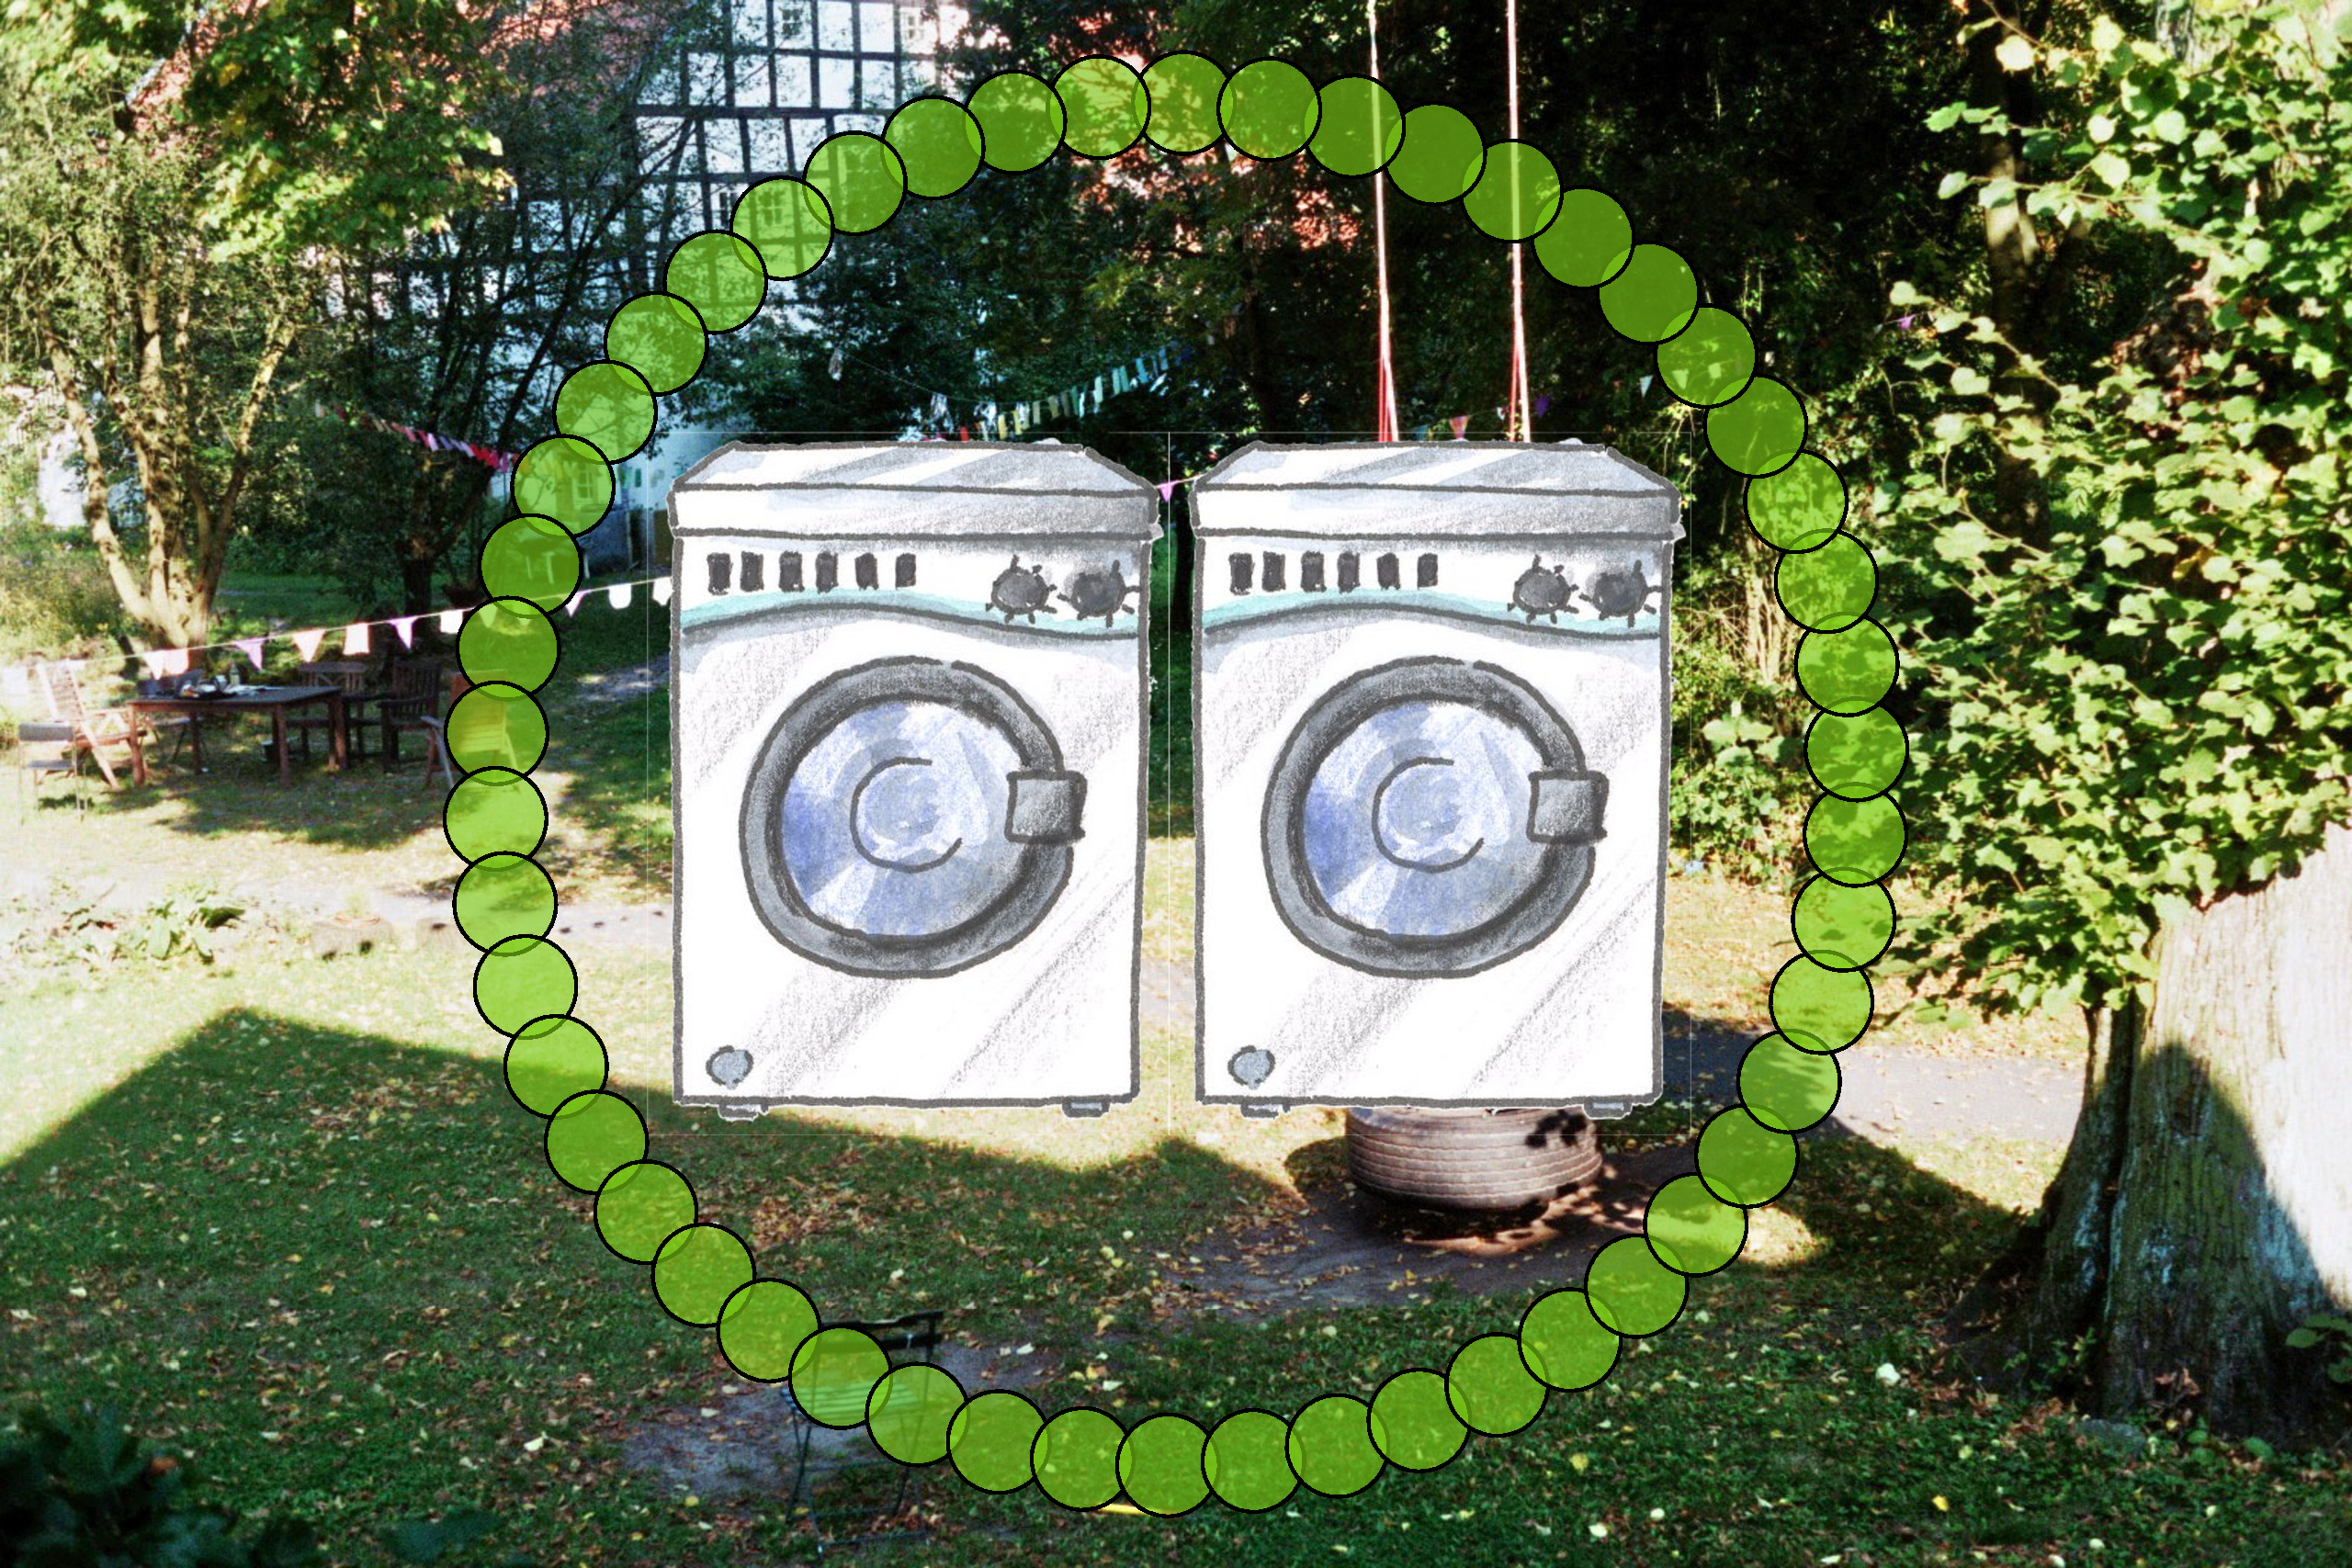
\includegraphics[width=0.9\textwidth]{Luhrmannhof50x2.pdf}
        \end{minipage}
        \hfill
        \begin{minipage}[t]{0.45\textwidth}
            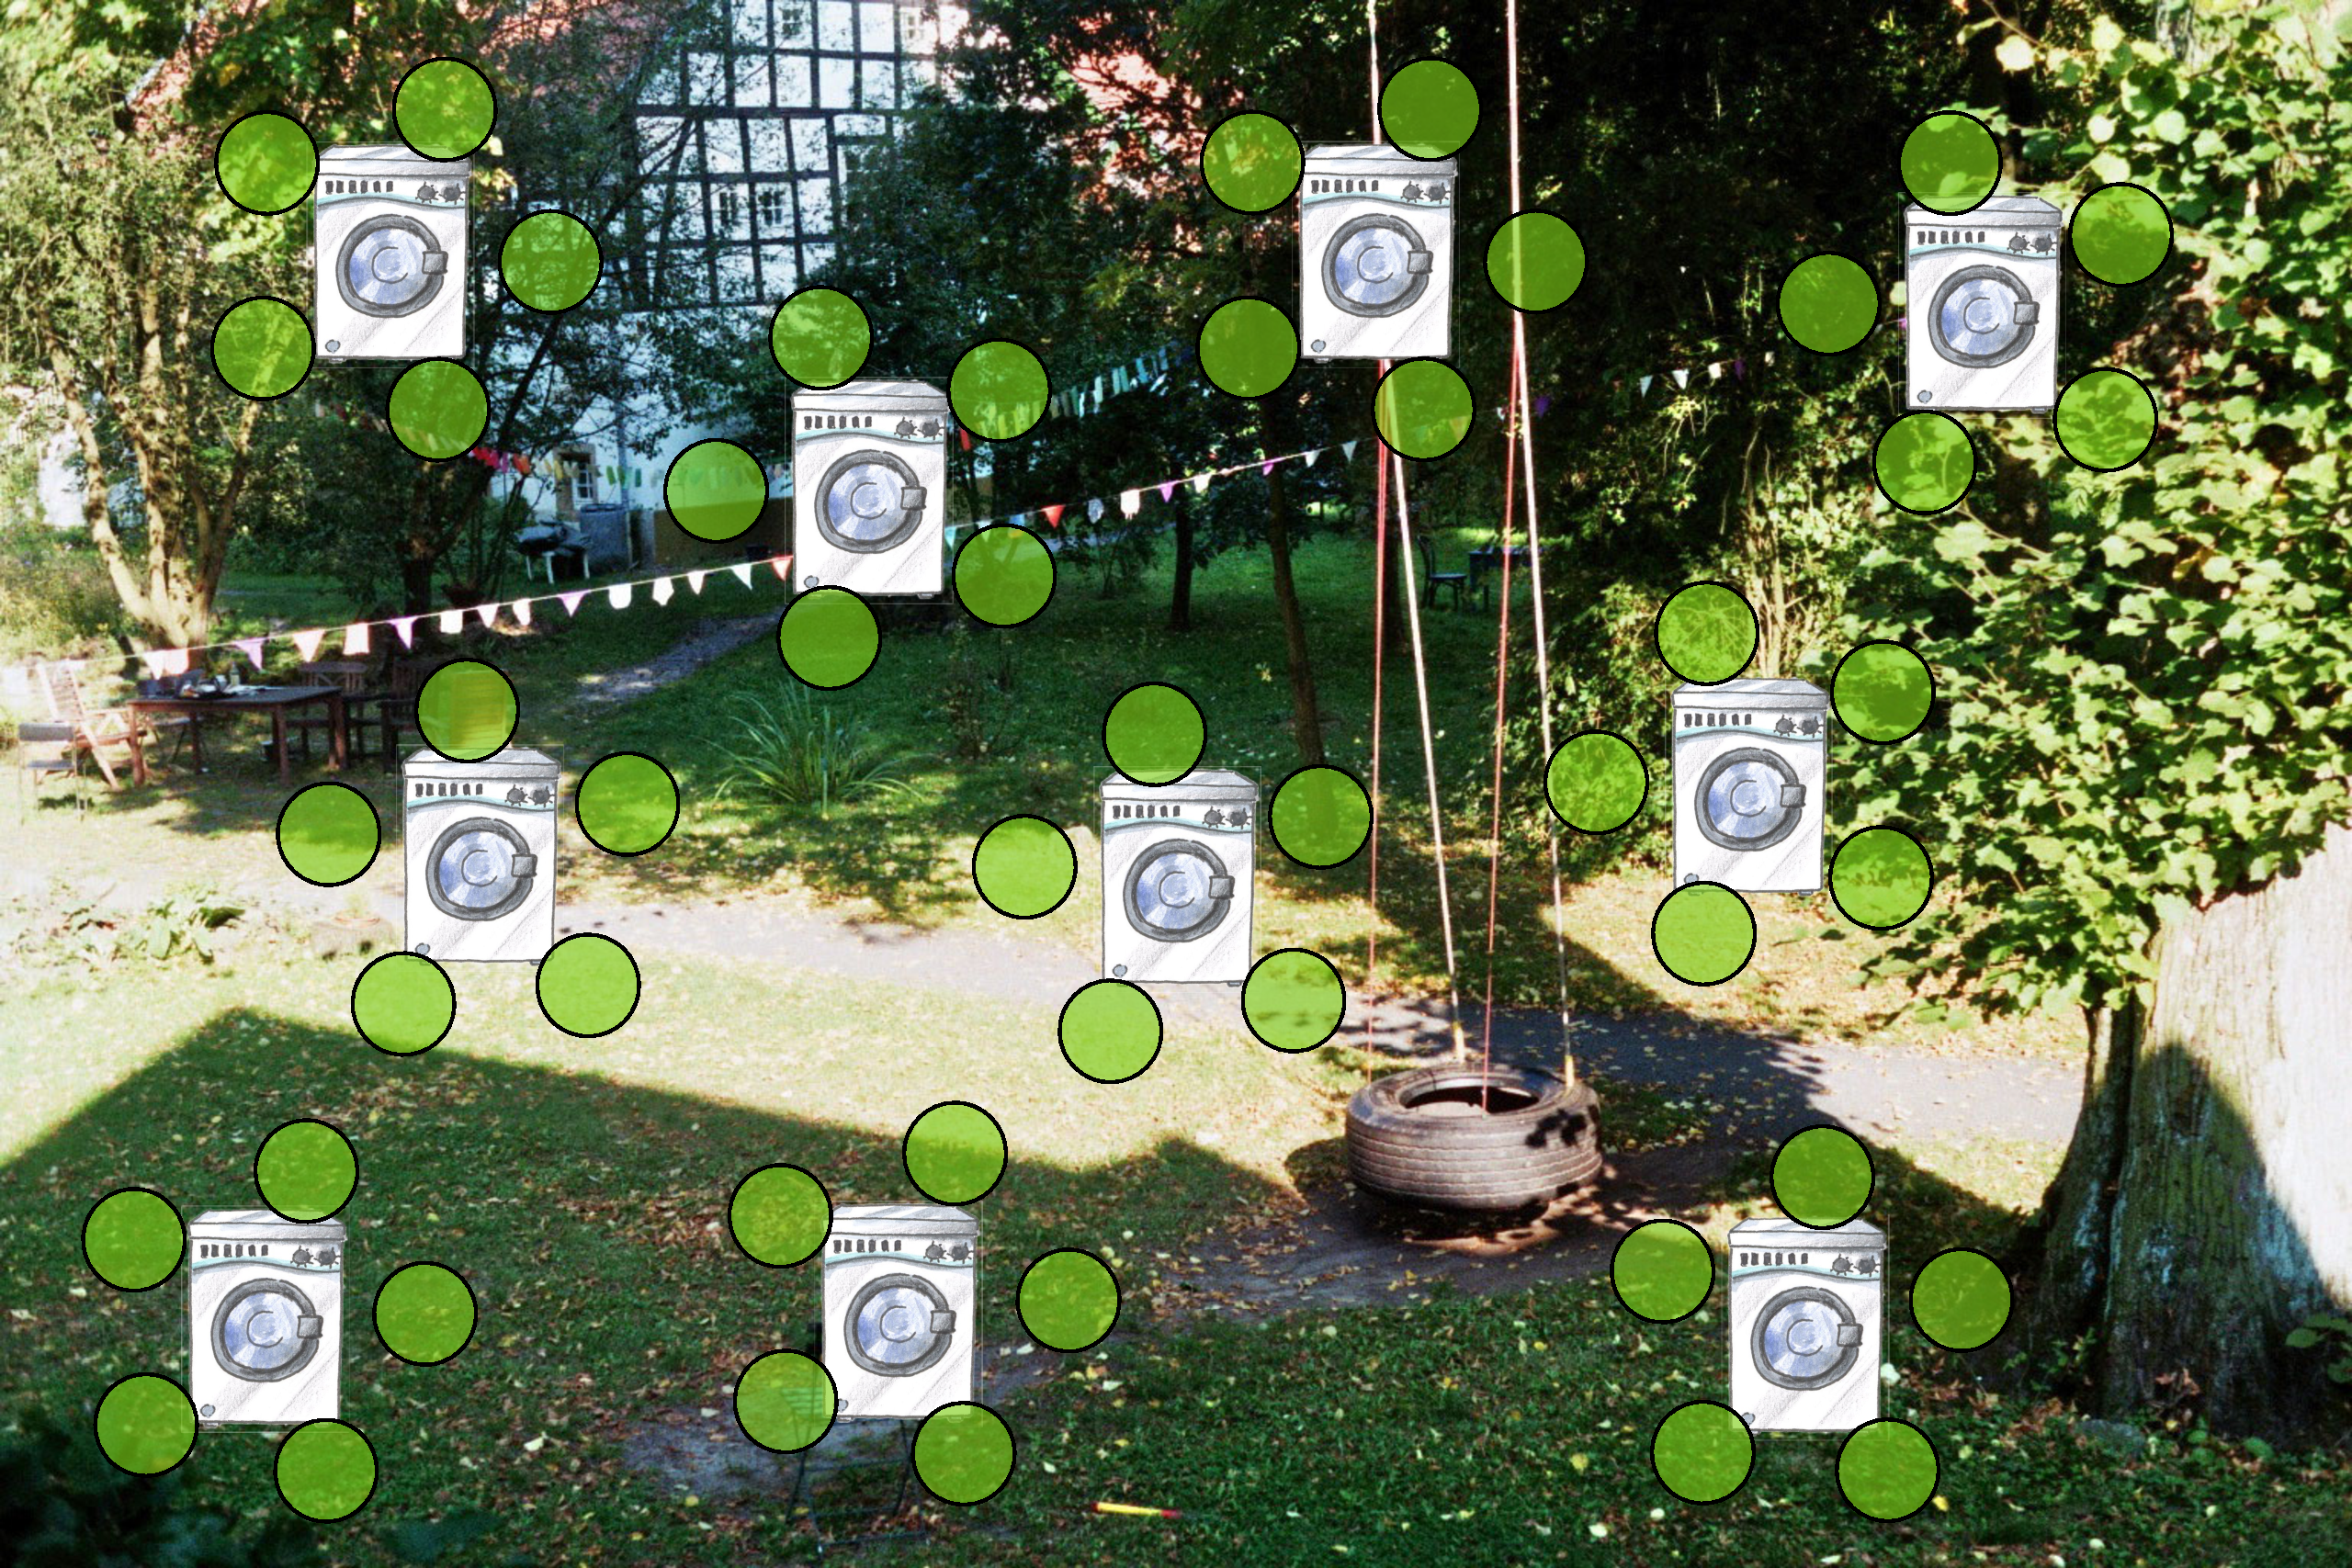
\includegraphics[width=0.9\textwidth]{Luhrmannhof10x5.pdf}
        \end{minipage}
        \pause
        \begin{itemize}
            % \item IZT: (S.12): $\t{max} = 8 - 10$ Jahre, $\n{max} = 2500$
            \item In einer Studie vom IÖW
                (2000)\footcite[S.57]{hirschl_produkte_2000} wird für einen
                durchschnittlichen Haushalt angegeben, "`[\dots] dass von einer
                weitestgehend vollständigen Ausnutzung des Leistungspotential
                von Hauhaltswaschmaschinen auszugehen ist."' 
                % $\t{max} = 14$ Jahre, $\n{max} = 2500$
                \pause
            \item[] $\Rightarrow$ Kein ökologischer Gewinn! (durch
                Nutzungsintensivierung)
                \pause
            \item Evtl. treten jedoch nicht berücksichtigte Effekte auf.
        \end{itemize}
    \end{frame}
\end{document}

